\documentclass[twoside]{book}

% Packages required by doxygen
\usepackage{calc}
\usepackage{doxygen}
\usepackage{graphicx}
\usepackage[utf8]{inputenc}
\usepackage{makeidx}
\usepackage{multicol}
\usepackage{multirow}
\usepackage{textcomp}
\usepackage[table]{xcolor}

% Font selection
\usepackage[T1]{fontenc}
\usepackage{mathptmx}
\usepackage[scaled=.90]{helvet}
\usepackage{courier}
\usepackage{amssymb}
\usepackage{sectsty}
\renewcommand{\familydefault}{\sfdefault}
\allsectionsfont{%
  \fontseries{bc}\selectfont%
  \color{darkgray}%
}
\renewcommand{\DoxyLabelFont}{%
  \fontseries{bc}\selectfont%
  \color{darkgray}%
}

% Page & text layout
\usepackage{geometry}
\geometry{%
  a4paper,%
  top=2.5cm,%
  bottom=2.5cm,%
  left=2.5cm,%
  right=2.5cm%
}
\tolerance=750
\hfuzz=15pt
\hbadness=750
\setlength{\emergencystretch}{15pt}
\setlength{\parindent}{0cm}
\setlength{\parskip}{0.2cm}
\makeatletter
\renewcommand{\paragraph}{%
  \@startsection{paragraph}{4}{0ex}{-1.0ex}{1.0ex}{%
    \normalfont\normalsize\bfseries\SS@parafont%
  }%
}
\renewcommand{\subparagraph}{%
  \@startsection{subparagraph}{5}{0ex}{-1.0ex}{1.0ex}{%
    \normalfont\normalsize\bfseries\SS@subparafont%
  }%
}
\makeatother

% Headers & footers
\usepackage{fancyhdr}
\pagestyle{fancyplain}
\fancyhead[LE]{\fancyplain{}{\bfseries\thepage}}
\fancyhead[CE]{\fancyplain{}{}}
\fancyhead[RE]{\fancyplain{}{\bfseries\leftmark}}
\fancyhead[LO]{\fancyplain{}{\bfseries\rightmark}}
\fancyhead[CO]{\fancyplain{}{}}
\fancyhead[RO]{\fancyplain{}{\bfseries\thepage}}
\fancyfoot[LE]{\fancyplain{}{}}
\fancyfoot[CE]{\fancyplain{}{}}
\fancyfoot[RE]{\fancyplain{}{\bfseries\scriptsize Generated on Mon Nov 28 2016 15\-:24\-:12 for My Project by Doxygen }}
\fancyfoot[LO]{\fancyplain{}{\bfseries\scriptsize Generated on Mon Nov 28 2016 15\-:24\-:12 for My Project by Doxygen }}
\fancyfoot[CO]{\fancyplain{}{}}
\fancyfoot[RO]{\fancyplain{}{}}
\renewcommand{\footrulewidth}{0.4pt}
\renewcommand{\chaptermark}[1]{%
  \markboth{#1}{}%
}
\renewcommand{\sectionmark}[1]{%
  \markright{\thesection\ #1}%
}

% Indices & bibliography
\usepackage{natbib}
\usepackage[titles]{tocloft}
\setcounter{tocdepth}{3}
\setcounter{secnumdepth}{5}
\makeindex

% Hyperlinks (required, but should be loaded last)
\usepackage{ifpdf}
\ifpdf
  \usepackage[pdftex,pagebackref=true]{hyperref}
\else
  \usepackage[ps2pdf,pagebackref=true]{hyperref}
\fi
\hypersetup{%
  colorlinks=true,%
  linkcolor=blue,%
  citecolor=blue,%
  unicode%
}

% Custom commands
\newcommand{\clearemptydoublepage}{%
  \newpage{\pagestyle{empty}\cleardoublepage}%
}


%===== C O N T E N T S =====

\begin{document}

% Titlepage & ToC
\hypersetup{pageanchor=false}
\pagenumbering{roman}
\begin{titlepage}
\vspace*{7cm}
\begin{center}%
{\Large My Project }\\
\vspace*{1cm}
{\large Generated by Doxygen 1.8.6}\\
\vspace*{0.5cm}
{\small Mon Nov 28 2016 15:24:12}\\
\end{center}
\end{titlepage}
\clearemptydoublepage
\tableofcontents
\clearemptydoublepage
\pagenumbering{arabic}
\hypersetup{pageanchor=true}

%--- Begin generated contents ---
\chapter{Class Index}
\section{Class List}
Here are the classes, structs, unions and interfaces with brief descriptions\-:\begin{DoxyCompactList}
\item\contentsline{section}{\hyperlink{classALogger}{A\-Logger} }{\pageref{classALogger}}{}
\item\contentsline{section}{\hyperlink{structRCS_1_1CanonCmd}{R\-C\-S\-::\-Canon\-Cmd} \\*\hyperlink{structRCS_1_1CanonCmd}{Canon\-Cmd} is the controller command structure }{\pageref{structRCS_1_1CanonCmd}}{}
\item\contentsline{section}{\hyperlink{structRCS_1_1CanonWorldModel}{R\-C\-S\-::\-Canon\-World\-Model} \\*\hyperlink{structRCS_1_1CanonWorldModel}{Canon\-World\-Model} describes the controller state. Includes reference to robot model }{\pageref{structRCS_1_1CanonWorldModel}}{}
\item\contentsline{section}{\hyperlink{classCAsioCrclServer}{C\-Asio\-Crcl\-Server} \\*Boost asio server which accepts new connections and starts a \hyperlink{namespaceCrcl}{Crcl} listener session. The \hyperlink{classCAsioCrclServer}{C\-Asio\-Crcl\-Server} class is based on the Boost Asio library which can process network communication asynchronously. Because C\-R\-C\-L data can only be received after a connection has been established, and because a connection can only be established after the name has been resolved, the various asynchronous operations are started in separate callback handlers. Thus in boost asio a callback to async\-\_\-connect() is then followed by a method call to the handler connect\-\_\-handler() which starts a new \hyperlink{namespaceCrcl}{Crcl} session. Readers can read more at\-: \href{http://theboostcpplibraries.com/boost.asio-network-programming}{\tt http\-://theboostcpplibraries.\-com/boost.\-asio-\/network-\/programming} The \hyperlink{classCAsioCrclServer}{C\-Asio\-Crcl\-Server} is divided into a number of main funcitons (e.\-g. wait for socket connection, handle new session by spawning new \hyperlink{classCAsioCrclSession}{C\-Asio\-Crcl\-Session}, repeat. These operations are done asynchronously on a separate thread with notification done by the boost asio io server and it is assumed to be thread-\/safe. The \hyperlink{classCAsioCrclServer}{C\-Asio\-Crcl\-Server} listens for connections on port 64444 and when a connection is initiated starts a new \hyperlink{namespaceCrcl}{Crcl} session to read xml messages from the devices }{\pageref{classCAsioCrclServer}}{}
\item\contentsline{section}{\hyperlink{classCAsioCrclSession}{C\-Asio\-Crcl\-Session} \\*Boost asio session ( which listens for each connected client). The \hyperlink{classCAsioCrclSession}{C\-Asio\-Crcl\-Session} listens for X\-M\-L messages and constructs. The \hyperlink{classCAsioCrclSession}{C\-Asio\-Crcl\-Session} uses mostly asynchronous operation for waiting, reading, and timeout of a socket connection. The operation is started by creating a session which starts an aynchronous thread, that is supplied I\-O communication events by the asio io service provider. After connection to the socket client, an \hyperlink{classCAsioCrclSession_ac7e0900916ab6de40bf546116d5e6d3e}{Start\-Aync\-Read()} that is paired with a timer is used to wait for communicatin from a socket. There is no trailing marker on C\-R\-C\-L X\-M\-L so any socket communication must be buffered and when a complete message has been received, it is pushed onto the inmsgs message queue. During the socket communication, a timeout can occur, which at this point only causes a new to be\-Start\-Aync\-Read() initiated. Because C\-R\-C\-L Xml does not have a trailing marker (e.\-g., zero or line feed), the \hyperlink{classCAsioCrclSession}{C\-Asio\-Crcl\-Session} must determine the trailing X\-M\-L tag to search for, by inspecting the communication for a X\-M\-L leading tag. It works, but is dubious. However, if the communicating socket is disconnected, an error is returned by asio, and the session is terminated cleanly. \par
 Useful web sites\-: }{\pageref{classCAsioCrclSession}}{}
\item\contentsline{section}{\hyperlink{structRCS_1_1CController}{R\-C\-S\-::\-C\-Controller} \\*The \hyperlink{structRCS_1_1CController}{C\-Controller} provides a collection for all the relevant controller pieces. The \hyperlink{structRCS_1_1CController}{C\-Controller} is the main controller class to collect all the references/pointers to instances in the project. A global instance of this class, called \char`\"{}\-Controller\char`\"{}, is created and is used throughout the code to reference various instances of control objects (e.\-g., kinematics, joint writer, joint reader, etc.) }{\pageref{structRCS_1_1CController}}{}
\item\contentsline{section}{\hyperlink{classCGlobals}{C\-Globals} \\*\hyperlink{classCGlobals}{C\-Globals} is a catch-\/all data structure for collecting global functions, extensions, parameters, etc. Functions here usually vary between windows and linux, or there is no easy mechanism in C++ to extend classes (e.\-g., string) like in C\# }{\pageref{classCGlobals}}{}
\item\contentsline{section}{\hyperlink{classRCS_1_1ChainRobotModel}{R\-C\-S\-::\-Chain\-Robot\-Model} }{\pageref{classRCS_1_1ChainRobotModel}}{}
\item\contentsline{section}{\hyperlink{classCJointReader}{C\-Joint\-Reader} \\*The \hyperlink{classCJointReader}{C\-Joint\-Reader} is a thread to accept joint update callbacks from R\-O\-S. Uses a ros node handle to tell roscore we are subscribing to joint\-\_\-state topic. Then, when joint updates occur, the callback routine is invoked and the latest joint values saved }{\pageref{classCJointReader}}{}
\item\contentsline{section}{\hyperlink{classCJointWriter}{C\-Joint\-Writer} \\*The \hyperlink{classCJointWriter}{C\-Joint\-Writer} is a thread to publish new joint values to R\-O\-S. Uses a ros node handle to tell roscore we are pusblishing to the joint\-\_\-path\-\_\-command topic. Then, when joint updates occur, these are published on joint\-\_\-path\-\_\-command the topic }{\pageref{classCJointWriter}}{}
\item\contentsline{section}{\hyperlink{classCLinkReader}{C\-Link\-Reader} \\*The \hyperlink{classCLinkReader}{C\-Link\-Reader} is a class that use the tf package from R\-O\-S to return latest pose of a link. Uses tf to find the latest time and base\-\_\-link and the desired link have changed. With the latest time it returns translation and orientation (quat) of the link. tf keeps track of a tree of coordinate frames. This tree changes over time, and tf stores a time snapshot for every transform (for up to 10 seconds by default) }{\pageref{classCLinkReader}}{}
\item\contentsline{section}{\hyperlink{classRCS_1_1CMessageQueue}{R\-C\-S\-::\-C\-Message\-Queue$<$ T $>$} \\*The \hyperlink{classRCS_1_1CMessageQueue}{C\-Message\-Queue} offers a mutexed front to a S\-T\-L/std deque. The queue is a L\-I\-F\-O data structure. Useful for safely sharing data between multiple threads }{\pageref{classRCS_1_1CMessageQueue}}{}
\item\contentsline{section}{\hyperlink{classCPrimitive}{C\-Primitive} }{\pageref{classCPrimitive}}{}
\item\contentsline{section}{\hyperlink{classCrcl_1_1CrclClientCmdInterface}{Crcl\-::\-Crcl\-Client\-Cmd\-Interface} \\*\hyperlink{classCrcl_1_1CrclClientCmdInterface}{Crcl\-Client\-Cmd\-Interface} generates \hyperlink{namespaceCrcl}{Crcl} X\-M\-L command message from to send to a \hyperlink{namespaceCrcl}{Crcl} server }{\pageref{classCrcl_1_1CrclClientCmdInterface}}{}
\item\contentsline{section}{\hyperlink{classCrcl_1_1CrclDelegateInterface}{Crcl\-::\-Crcl\-Delegate\-Interface} \\*\hyperlink{classCrcl_1_1CrclDelegateInterface}{Crcl\-Delegate\-Interface} parses \hyperlink{namespaceCrcl}{Crcl} commands and interprets into robot motion. \href{https://github.com/usnistgov/crcl/blob/master/doc/Reference.md}{\tt https\-://github.\-com/usnistgov/crcl/blob/master/doc/\-Reference.\-md} }{\pageref{classCrcl_1_1CrclDelegateInterface}}{}
\item\contentsline{section}{\hyperlink{structCrcl_1_1CrclStatus}{Crcl\-::\-Crcl\-Status} \\*\hyperlink{structCrcl_1_1CrclStatus}{Crcl\-Status} is a class that encapsulates all the C\-R\-C\-L information. All lot of the knowledge is converting R\-O\-S oriented \hyperlink{namespaceRCS}{R\-C\-S} data into codesynthesis \hyperlink{namespaceCrcl}{Crcl} representation and vice versa. \hyperlink{structCrcl_1_1CrclStatus}{Crcl\-Status} maintains the unit a crcl session uses to transmit robot commands, latest robot status, etc }{\pageref{structCrcl_1_1CrclStatus}}{}
\item\contentsline{section}{\hyperlink{classCrcl_1_1CrclStatusMsgInterface}{Crcl\-::\-Crcl\-Status\-Msg\-Interface} \\*\hyperlink{classCrcl_1_1CrclStatusMsgInterface}{Crcl\-Status\-Msg\-Interface} parses a \hyperlink{namespaceCrcl}{Crcl} X\-M\-L status message from a \hyperlink{namespaceCrcl}{Crcl} server }{\pageref{classCrcl_1_1CrclStatusMsgInterface}}{}
\item\contentsline{section}{\hyperlink{classCRvizMarker}{C\-Rviz\-Marker} \\*The \hyperlink{classCRvizMarker}{C\-Rviz\-Marker} provides a C++ class to send markers to rviz. Note you must manually add the rviz subscribe to marker messages. Read here for explanation \href{http://answers.ros.org/question/11135/plotting-a-markerarray-of-spheres-with-rviz/}{\tt http\-://answers.\-ros.\-org/question/11135/plotting-\/a-\/markerarray-\/of-\/spheres-\/with-\/rviz/} }{\pageref{classCRvizMarker}}{}
\item\contentsline{section}{\hyperlink{classCTrajectory}{C\-Trajectory} }{\pageref{classCTrajectory}}{}
\item\contentsline{section}{\hyperlink{classDummyKinematics}{Dummy\-Kinematics} \\*instantiates the \hyperlink{classIKinematics}{I\-Kinematics} abstract class and fills in the pure virtual functions with dummy methods }{\pageref{classDummyKinematics}}{}
\item\contentsline{section}{\hyperlink{structCrcl_1_1GripperStatus}{Crcl\-::\-Gripper\-Status} \\*\hyperlink{structCrcl_1_1GripperStatus}{Gripper\-Status} dummy class for future gripper information }{\pageref{structCrcl_1_1GripperStatus}}{}
\item\contentsline{section}{\hyperlink{classIKinematics}{I\-Kinematics} \\*The \hyperlink{classIKinematics}{I\-Kinematics} provides is an abstract class with pure virtual functions that are overriden by actual kinematic implementations }{\pageref{classIKinematics}}{}
\item\contentsline{section}{\hyperlink{classRCS_1_1IRate}{R\-C\-S\-::\-I\-Rate} \\*\hyperlink{classRCS_1_1IRate}{I\-Rate} is an interface class for defining the allowed motion rates }{\pageref{classRCS_1_1IRate}}{}
\item\contentsline{section}{\hyperlink{structCrcl_1_1JointReport}{Crcl\-::\-Joint\-Report} \\*\hyperlink{structCrcl_1_1JointReport}{Joint\-Report} dummy class for future customization of \hyperlink{namespaceCrcl}{Crcl} status reports }{\pageref{structCrcl_1_1JointReport}}{}
\item\contentsline{section}{\hyperlink{classMotionControl}{Motion\-Control} \\*\hyperlink{classMotionControl}{Motion\-Control} is a class that contains some useful motion control methods }{\pageref{classMotionControl}}{}
\item\contentsline{section}{\hyperlink{classMoveitKinematics}{Moveit\-Kinematics} \\*instantiates the \hyperlink{classIKinematics}{I\-Kinematics} abstract class and fills in the pure virtual functions with Moveit kinematic methods }{\pageref{classMoveitKinematics}}{}
\item\contentsline{section}{\hyperlink{classMoveitPlanning}{Moveit\-Planning} }{\pageref{classMoveitPlanning}}{}
\item\contentsline{section}{\hyperlink{classRCSInterpreter}{R\-C\-S\-Interpreter} \\*\hyperlink{classRCSInterpreter}{R\-C\-S\-Interpreter} parses a \hyperlink{namespaceRCS}{R\-C\-S} command and generates robot motion commands }{\pageref{classRCSInterpreter}}{}
\item\contentsline{section}{\hyperlink{structRCS_1_1RdfJoint}{R\-C\-S\-::\-Rdf\-Joint} }{\pageref{structRCS_1_1RdfJoint}}{}
\item\contentsline{section}{\hyperlink{classRCS_1_1RobotProgram}{R\-C\-S\-::\-Robot\-Program} \\*The \hyperlink{classRCS_1_1RobotProgram}{Robot\-Program} is a thread to handle crcl programs. \hyperlink{namespaceCrcl}{Crcl} programs are not in fact legitimate, however, debugging and verification are assisted by programs. However, program as in the \hyperlink{namespaceCrcl}{Crcl} X\-S\-D specification, so it doesn't hurt to handle. They require special handling as only one command should be done at a time. Uses codesynthesis to parse \hyperlink{namespaceCrcl}{Crcl} xml into C++ data structures }{\pageref{classRCS_1_1RobotProgram}}{}
\item\contentsline{section}{\hyperlink{classRCS_1_1RobotStatus}{R\-C\-S\-::\-Robot\-Status} \\*The \hyperlink{classRCS_1_1RobotStatus}{Robot\-Status} is a thread that reads the status of the robot and updates the world model. The \hyperlink{classRCS_1_1RobotStatus}{Robot\-Status} is a separate thread that reads the robot status using R\-O\-S communication mechanisms and updates the controller world model based on these values. Currently, it uses an instance of the class Joint\-Reader to read joint values from the controller. It uses a Kinematics pointer reference to compute the current robot pose using the forward kinematics (F\-K) routine. It also uses a Crcl\-Delegate pointer reference to update the status reported by C\-R\-C\-L }{\pageref{classRCS_1_1RobotStatus}}{}
\item\contentsline{section}{\hyperlink{classRosKinematics}{Ros\-Kinematics} \\*instantiates the \hyperlink{classIKinematics}{I\-Kinematics} abstract class and fills in the pure virtual functions with Descartes kinematic methods }{\pageref{classRosKinematics}}{}
\item\contentsline{section}{\hyperlink{classRCS_1_1Thread}{R\-C\-S\-::\-Thread} \\*\hyperlink{classRCS_1_1Thread}{Thread} is an \hyperlink{namespaceRCS}{R\-C\-S} ulapi equivalent for a timed thread. Given a cycle time, the thread provides a wait function to sleep to exactly the amount of the thread cycle time. It keeps track of busy/idle time for diagnostic purposes. \par
 Notes\-: \href{https://www.quantnet.com/threads/c-multithreading-in-boost.10028/}{\tt https\-://www.\-quantnet.\-com/threads/c-\/multithreading-\/in-\/boost.\-10028/} }{\pageref{classRCS_1_1Thread}}{}
\item\contentsline{section}{\hyperlink{classRCS_1_1Timer}{R\-C\-S\-::\-Timer} \\*\hyperlink{classRCS_1_1Timer}{Timer} is a general-\/purpose timer. The \hyperlink{classRCS_1_1Timer}{Timer} is a general-\/purpose timer, which can be used for waiting until a synchronous time tick, sleep for any period at all, or to obtain a time in system clock ticks from creation of the timer }{\pageref{classRCS_1_1Timer}}{}
\item\contentsline{section}{\hyperlink{classTrajectoryMaker}{Trajectory\-Maker} \\*\hyperlink{classTrajectoryMaker}{Trajectory\-Maker} generates simple trapezoidal velocities. Will accept non-\/zero final velocity }{\pageref{classTrajectoryMaker}}{}
\end{DoxyCompactList}

\chapter{File Index}
\section{File List}
Here is a list of all files with brief descriptions\-:\begin{DoxyCompactList}
\item\contentsline{section}{/usr/local/michalos/nistfanuc\-\_\-ws/src/nist\-\_\-fanuc/include/nist\-\_\-fanuc/\hyperlink{arm__kinematics_8h}{arm\-\_\-kinematics.\-h} }{\pageref{arm__kinematics_8h}}{}
\item\contentsline{section}{/usr/local/michalos/nistfanuc\-\_\-ws/src/nist\-\_\-fanuc/include/nist\-\_\-fanuc/\hyperlink{Checkerboard_8h}{Checkerboard.\-h} }{\pageref{Checkerboard_8h}}{}
\item\contentsline{section}{/usr/local/michalos/nistfanuc\-\_\-ws/src/nist\-\_\-fanuc/include/nist\-\_\-fanuc/\hyperlink{Checkers_8h}{Checkers.\-h} }{\pageref{Checkers_8h}}{}
\item\contentsline{section}{/usr/local/michalos/nistfanuc\-\_\-ws/src/nist\-\_\-fanuc/include/nist\-\_\-fanuc/\hyperlink{Communication_8h}{Communication.\-h} }{\pageref{Communication_8h}}{}
\item\contentsline{section}{/usr/local/michalos/nistfanuc\-\_\-ws/src/nist\-\_\-fanuc/include/nist\-\_\-fanuc/\hyperlink{Controller_8h}{Controller.\-h} }{\pageref{Controller_8h}}{}
\item\contentsline{section}{/usr/local/michalos/nistfanuc\-\_\-ws/src/nist\-\_\-fanuc/include/nist\-\_\-fanuc/\hyperlink{Conversions_8h}{Conversions.\-h} }{\pageref{Conversions_8h}}{}
\item\contentsline{section}{/usr/local/michalos/nistfanuc\-\_\-ws/src/nist\-\_\-fanuc/include/nist\-\_\-fanuc/\hyperlink{CsvLogging_8h}{Csv\-Logging.\-h} }{\pageref{CsvLogging_8h}}{}
\item\contentsline{section}{/usr/local/michalos/nistfanuc\-\_\-ws/src/nist\-\_\-fanuc/include/nist\-\_\-fanuc/\hyperlink{Debug_8h}{Debug.\-h} }{\pageref{Debug_8h}}{}
\item\contentsline{section}{/usr/local/michalos/nistfanuc\-\_\-ws/src/nist\-\_\-fanuc/include/nist\-\_\-fanuc/\hyperlink{Demo_8h}{Demo.\-h} }{\pageref{Demo_8h}}{}
\item\contentsline{section}{/usr/local/michalos/nistfanuc\-\_\-ws/src/nist\-\_\-fanuc/include/nist\-\_\-fanuc/\hyperlink{fanuc__lrmate200id_8h}{fanuc\-\_\-lrmate200id.\-h} }{\pageref{fanuc__lrmate200id_8h}}{}
\item\contentsline{section}{/usr/local/michalos/nistfanuc\-\_\-ws/src/nist\-\_\-fanuc/include/nist\-\_\-fanuc/\hyperlink{Globals_8h}{Globals.\-h} }{\pageref{Globals_8h}}{}
\item\contentsline{section}{/usr/local/michalos/nistfanuc\-\_\-ws/src/nist\-\_\-fanuc/include/nist\-\_\-fanuc/\hyperlink{Gripper_8h}{Gripper.\-h} }{\pageref{Gripper_8h}}{}
\item\contentsline{section}{/usr/local/michalos/nistfanuc\-\_\-ws/src/nist\-\_\-fanuc/include/nist\-\_\-fanuc/\hyperlink{ikfast_8h}{ikfast.\-h} }{\pageref{ikfast_8h}}{}
\item\contentsline{section}{/usr/local/michalos/nistfanuc\-\_\-ws/src/nist\-\_\-fanuc/include/nist\-\_\-fanuc/\hyperlink{Kinematics_8h}{Kinematics.\-h} }{\pageref{Kinematics_8h}}{}
\item\contentsline{section}{/usr/local/michalos/nistfanuc\-\_\-ws/src/nist\-\_\-fanuc/include/nist\-\_\-fanuc/\hyperlink{MotionControl_8h}{Motion\-Control.\-h} }{\pageref{MotionControl_8h}}{}
\item\contentsline{section}{/usr/local/michalos/nistfanuc\-\_\-ws/src/nist\-\_\-fanuc/include/nist\-\_\-fanuc/\hyperlink{nist__fanuc_8h}{nist\-\_\-fanuc.\-h} }{\pageref{nist__fanuc_8h}}{}
\item\contentsline{section}{/usr/local/michalos/nistfanuc\-\_\-ws/src/nist\-\_\-fanuc/include/nist\-\_\-fanuc/\hyperlink{RCS_8h}{R\-C\-S.\-h} }{\pageref{RCS_8h}}{}
\item\contentsline{section}{/usr/local/michalos/nistfanuc\-\_\-ws/src/nist\-\_\-fanuc/include/nist\-\_\-fanuc/\hyperlink{RCSInterpreter_8h}{R\-C\-S\-Interpreter.\-h} }{\pageref{RCSInterpreter_8h}}{}
\item\contentsline{section}{/usr/local/michalos/nistfanuc\-\_\-ws/src/nist\-\_\-fanuc/include/nist\-\_\-fanuc/\hyperlink{RosConversions_8h}{Ros\-Conversions.\-h} }{\pageref{RosConversions_8h}}{}
\item\contentsline{section}{/usr/local/michalos/nistfanuc\-\_\-ws/src/nist\-\_\-fanuc/include/nist\-\_\-fanuc/\hyperlink{RosSetup_8h}{Ros\-Setup.\-h} }{\pageref{RosSetup_8h}}{}
\item\contentsline{section}{/usr/local/michalos/nistfanuc\-\_\-ws/src/nist\-\_\-fanuc/include/nist\-\_\-fanuc/\hyperlink{RvizMarker_8h}{Rviz\-Marker.\-h} }{\pageref{RvizMarker_8h}}{}
\item\contentsline{section}{/usr/local/michalos/nistfanuc\-\_\-ws/src/nist\-\_\-fanuc/include/nist\-\_\-fanuc/\hyperlink{Scene_8h}{Scene.\-h} }{\pageref{Scene_8h}}{}
\item\contentsline{section}{/usr/local/michalos/nistfanuc\-\_\-ws/src/nist\-\_\-fanuc/include/nist\-\_\-fanuc/\hyperlink{StackTrace_8h}{Stack\-Trace.\-h} }{\pageref{StackTrace_8h}}{}
\item\contentsline{section}{/usr/local/michalos/nistfanuc\-\_\-ws/src/nist\-\_\-fanuc/include/nist\-\_\-fanuc/\hyperlink{Test_8h}{Test.\-h} }{\pageref{Test_8h}}{}
\item\contentsline{section}{/usr/local/michalos/nistfanuc\-\_\-ws/src/nist\-\_\-fanuc/include/nist\-\_\-fanuc/\hyperlink{trajectoryMaker_8h}{trajectory\-Maker.\-h} }{\pageref{trajectoryMaker_8h}}{}
\item\contentsline{section}{/usr/local/michalos/nistfanuc\-\_\-ws/src/nist\-\_\-fanuc/include/nist\-\_\-fanuc/\-I\-K\-F\-A\-S\-T/\hyperlink{include_2nist__fanuc_2IKFAST_2Kinematics_8cpp}{Kinematics.\-cpp} }{\pageref{include_2nist__fanuc_2IKFAST_2Kinematics_8cpp}}{}
\item\contentsline{section}{/usr/local/michalos/nistfanuc\-\_\-ws/src/nist\-\_\-fanuc/include/nist\-\_\-fanuc/\-I\-K\-F\-A\-S\-T/\hyperlink{IKFAST_2Kinematics_8h}{Kinematics.\-h} }{\pageref{IKFAST_2Kinematics_8h}}{}
\item\contentsline{section}{/usr/local/michalos/nistfanuc\-\_\-ws/src/nist\-\_\-fanuc/include/nist\-\_\-fanuc/\-N\-I\-S\-T/\hyperlink{BLogging_8h}{B\-Logging.\-h} }{\pageref{BLogging_8h}}{}
\item\contentsline{section}{/usr/local/michalos/nistfanuc\-\_\-ws/src/nist\-\_\-fanuc/include/nist\-\_\-fanuc/\-N\-I\-S\-T/\hyperlink{RCSMsgQueue_8h}{R\-C\-S\-Msg\-Queue.\-h} }{\pageref{RCSMsgQueue_8h}}{}
\item\contentsline{section}{/usr/local/michalos/nistfanuc\-\_\-ws/src/nist\-\_\-fanuc/include/nist\-\_\-fanuc/\-N\-I\-S\-T/\hyperlink{RCSMsgQueueThread_8h}{R\-C\-S\-Msg\-Queue\-Thread.\-h} }{\pageref{RCSMsgQueueThread_8h}}{}
\item\contentsline{section}{/usr/local/michalos/nistfanuc\-\_\-ws/src/nist\-\_\-fanuc/include/nist\-\_\-fanuc/\-N\-I\-S\-T/\hyperlink{RCSThreadTemplate_8h}{R\-C\-S\-Thread\-Template.\-h} }{\pageref{RCSThreadTemplate_8h}}{}
\item\contentsline{section}{/usr/local/michalos/nistfanuc\-\_\-ws/src/nist\-\_\-fanuc/include/nist\-\_\-fanuc/\-N\-I\-S\-T/\hyperlink{RCSTimer_8h}{R\-C\-S\-Timer.\-h} }{\pageref{RCSTimer_8h}}{}
\item\contentsline{section}{/usr/local/michalos/nistfanuc\-\_\-ws/src/nist\-\_\-fanuc/src/\hyperlink{arm__kinematics_8cpp}{arm\-\_\-kinematics.\-cpp} }{\pageref{arm__kinematics_8cpp}}{}
\item\contentsline{section}{/usr/local/michalos/nistfanuc\-\_\-ws/src/nist\-\_\-fanuc/src/\hyperlink{BLogging_8cpp}{B\-Logging.\-cpp} }{\pageref{BLogging_8cpp}}{}
\item\contentsline{section}{/usr/local/michalos/nistfanuc\-\_\-ws/src/nist\-\_\-fanuc/src/\hyperlink{Communication_8cpp}{Communication.\-cpp} }{\pageref{Communication_8cpp}}{}
\item\contentsline{section}{/usr/local/michalos/nistfanuc\-\_\-ws/src/nist\-\_\-fanuc/src/\hyperlink{Controller_8cpp}{Controller.\-cpp} }{\pageref{Controller_8cpp}}{}
\item\contentsline{section}{/usr/local/michalos/nistfanuc\-\_\-ws/src/nist\-\_\-fanuc/src/\hyperlink{Conversions_8cpp}{Conversions.\-cpp} }{\pageref{Conversions_8cpp}}{}
\item\contentsline{section}{/usr/local/michalos/nistfanuc\-\_\-ws/src/nist\-\_\-fanuc/src/\hyperlink{CsvLogging_8cpp}{Csv\-Logging.\-cpp} }{\pageref{CsvLogging_8cpp}}{}
\item\contentsline{section}{/usr/local/michalos/nistfanuc\-\_\-ws/src/nist\-\_\-fanuc/src/\hyperlink{Demo_8cpp}{Demo.\-cpp} }{\pageref{Demo_8cpp}}{}
\item\contentsline{section}{/usr/local/michalos/nistfanuc\-\_\-ws/src/nist\-\_\-fanuc/src/\hyperlink{fanuc__lrmate200id_8cpp}{fanuc\-\_\-lrmate200id.\-cpp} }{\pageref{fanuc__lrmate200id_8cpp}}{}
\item\contentsline{section}{/usr/local/michalos/nistfanuc\-\_\-ws/src/nist\-\_\-fanuc/src/\hyperlink{fanuc__lrmate200id__manipulator__ikfast__solver_8cpp}{fanuc\-\_\-lrmate200id\-\_\-manipulator\-\_\-ikfast\-\_\-solver.\-cpp} }{\pageref{fanuc__lrmate200id__manipulator__ikfast__solver_8cpp}}{}
\item\contentsline{section}{/usr/local/michalos/nistfanuc\-\_\-ws/src/nist\-\_\-fanuc/src/\hyperlink{Globals_8cpp}{Globals.\-cpp} }{\pageref{Globals_8cpp}}{}
\item\contentsline{section}{/usr/local/michalos/nistfanuc\-\_\-ws/src/nist\-\_\-fanuc/src/\hyperlink{src_2Kinematics_8cpp}{Kinematics.\-cpp} }{\pageref{src_2Kinematics_8cpp}}{}
\item\contentsline{section}{/usr/local/michalos/nistfanuc\-\_\-ws/src/nist\-\_\-fanuc/src/\hyperlink{MotionControl_8cpp}{Motion\-Control.\-cpp} }{\pageref{MotionControl_8cpp}}{}
\item\contentsline{section}{/usr/local/michalos/nistfanuc\-\_\-ws/src/nist\-\_\-fanuc/src/\hyperlink{nist__fanuc_8cpp}{nist\-\_\-fanuc.\-cpp} }{\pageref{nist__fanuc_8cpp}}{}
\item\contentsline{section}{/usr/local/michalos/nistfanuc\-\_\-ws/src/nist\-\_\-fanuc/src/\hyperlink{RCS_8cpp}{R\-C\-S.\-cpp} }{\pageref{RCS_8cpp}}{}
\item\contentsline{section}{/usr/local/michalos/nistfanuc\-\_\-ws/src/nist\-\_\-fanuc/src/\hyperlink{RCSInterpreter_8cpp}{R\-C\-S\-Interpreter.\-cpp} }{\pageref{RCSInterpreter_8cpp}}{}
\item\contentsline{section}{/usr/local/michalos/nistfanuc\-\_\-ws/src/nist\-\_\-fanuc/src/\hyperlink{RosSetup_8cpp}{Ros\-Setup.\-cpp} }{\pageref{RosSetup_8cpp}}{}
\item\contentsline{section}{/usr/local/michalos/nistfanuc\-\_\-ws/src/nist\-\_\-fanuc/src/\hyperlink{RvizMarker_8cpp}{Rviz\-Marker.\-cpp} }{\pageref{RvizMarker_8cpp}}{}
\item\contentsline{section}{/usr/local/michalos/nistfanuc\-\_\-ws/src/nist\-\_\-fanuc/src/\hyperlink{Scene_8cpp}{Scene.\-cpp} }{\pageref{Scene_8cpp}}{}
\item\contentsline{section}{/usr/local/michalos/nistfanuc\-\_\-ws/src/nist\-\_\-fanuc/src/\hyperlink{trajectoryMaker_8cpp}{trajectory\-Maker.\-cpp} }{\pageref{trajectoryMaker_8cpp}}{}
\end{DoxyCompactList}

\chapter{Class Documentation}
\hypertarget{structgomotion_1_1go__motion__circular__params}{\section{gomotion\-:\-:go\-\_\-motion\-\_\-circular\-\_\-params Struct Reference}
\label{structgomotion_1_1go__motion__circular__params}\index{gomotion\-::go\-\_\-motion\-\_\-circular\-\_\-params@{gomotion\-::go\-\_\-motion\-\_\-circular\-\_\-params}}
}


{\ttfamily \#include $<$gomotion.\-h$>$}



Collaboration diagram for gomotion\-:\-:go\-\_\-motion\-\_\-circular\-\_\-params\-:\nopagebreak
\begin{figure}[H]
\begin{center}
\leavevmode
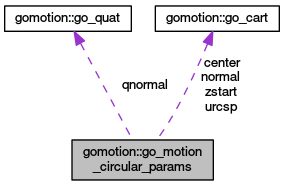
\includegraphics[width=285pt]{da/d58/structgomotion_1_1go__motion__circular__params__coll__graph}
\end{center}
\end{figure}
\subsection*{Data Fields}
\begin{DoxyCompactItemize}
\item 
\hyperlink{structgomotion_1_1go__cart}{go\-\_\-cart} \hyperlink{structgomotion_1_1go__motion__circular__params_afcf8dda6a72f29ce49a61130adbf3971}{center}
\item 
\hyperlink{structgomotion_1_1go__cart}{go\-\_\-cart} \hyperlink{structgomotion_1_1go__motion__circular__params_af933e19d1dba3641d570a3aa42b9969b}{normal}
\item 
\hyperlink{structgomotion_1_1go__quat}{go\-\_\-quat} \hyperlink{structgomotion_1_1go__motion__circular__params_abd5283624621e9fb218671e9996eb3c3}{qnormal}
\item 
\hyperlink{structgomotion_1_1go__cart}{go\-\_\-cart} \hyperlink{structgomotion_1_1go__motion__circular__params_ab97f8ccebf3ca78e2be4a4adfe9c9e8c}{urcsp}
\item 
\hyperlink{gotypes_8h_afd666a2393eebd71ee455846ac9def9b}{go\-\_\-real} \hyperlink{structgomotion_1_1go__motion__circular__params_aeee40430ac2667fef1fc6eba842427b7}{rstart}
\item 
\hyperlink{structgomotion_1_1go__cart}{go\-\_\-cart} \hyperlink{structgomotion_1_1go__motion__circular__params_a3638d197aac3d27862052befae408e94}{zstart}
\item 
\hyperlink{gotypes_8h_afd666a2393eebd71ee455846ac9def9b}{go\-\_\-real} \hyperlink{structgomotion_1_1go__motion__circular__params_a03f65f0ef19c2d9e83d05de75fe9fd3f}{thtot}
\item 
\hyperlink{gotypes_8h_afd666a2393eebd71ee455846ac9def9b}{go\-\_\-real} \hyperlink{structgomotion_1_1go__motion__circular__params_a576992f878d73c0771e072fe37438f4f}{rtot}
\item 
\hyperlink{gotypes_8h_afd666a2393eebd71ee455846ac9def9b}{go\-\_\-real} \hyperlink{structgomotion_1_1go__motion__circular__params_a1572625c5322b3ace560429703948191}{ztot}
\item 
\hyperlink{gotypes_8h_afd666a2393eebd71ee455846ac9def9b}{go\-\_\-real} \hyperlink{structgomotion_1_1go__motion__circular__params_a4436b498d123ce3776166eb75e8efcd5}{stotinv}
\item 
\hyperlink{gotypes_8h_a7d30f606bb0f58ffe2b3bd71e5c8af5c}{go\-\_\-integer} \hyperlink{structgomotion_1_1go__motion__circular__params_a2d8430003302e61cb95c2a0c75e60037}{turns}
\end{DoxyCompactItemize}


\subsection{Field Documentation}
\hypertarget{structgomotion_1_1go__motion__circular__params_afcf8dda6a72f29ce49a61130adbf3971}{\index{gomotion\-::go\-\_\-motion\-\_\-circular\-\_\-params@{gomotion\-::go\-\_\-motion\-\_\-circular\-\_\-params}!center@{center}}
\index{center@{center}!gomotion::go_motion_circular_params@{gomotion\-::go\-\_\-motion\-\_\-circular\-\_\-params}}
\subsubsection[{center}]{\setlength{\rightskip}{0pt plus 5cm}{\bf go\-\_\-cart} gomotion\-::go\-\_\-motion\-\_\-circular\-\_\-params\-::center}}\label{structgomotion_1_1go__motion__circular__params_afcf8dda6a72f29ce49a61130adbf3971}
The vector to the circle center. \hypertarget{structgomotion_1_1go__motion__circular__params_af933e19d1dba3641d570a3aa42b9969b}{\index{gomotion\-::go\-\_\-motion\-\_\-circular\-\_\-params@{gomotion\-::go\-\_\-motion\-\_\-circular\-\_\-params}!normal@{normal}}
\index{normal@{normal}!gomotion::go_motion_circular_params@{gomotion\-::go\-\_\-motion\-\_\-circular\-\_\-params}}
\subsubsection[{normal}]{\setlength{\rightskip}{0pt plus 5cm}{\bf go\-\_\-cart} gomotion\-::go\-\_\-motion\-\_\-circular\-\_\-params\-::normal}}\label{structgomotion_1_1go__motion__circular__params_af933e19d1dba3641d570a3aa42b9969b}
The normal vector that defines the plane of the circle. \hypertarget{structgomotion_1_1go__motion__circular__params_abd5283624621e9fb218671e9996eb3c3}{\index{gomotion\-::go\-\_\-motion\-\_\-circular\-\_\-params@{gomotion\-::go\-\_\-motion\-\_\-circular\-\_\-params}!qnormal@{qnormal}}
\index{qnormal@{qnormal}!gomotion::go_motion_circular_params@{gomotion\-::go\-\_\-motion\-\_\-circular\-\_\-params}}
\subsubsection[{qnormal}]{\setlength{\rightskip}{0pt plus 5cm}{\bf go\-\_\-quat} gomotion\-::go\-\_\-motion\-\_\-circular\-\_\-params\-::qnormal}}\label{structgomotion_1_1go__motion__circular__params_abd5283624621e9fb218671e9996eb3c3}
The normal vector expressed as a unit rotation. \hypertarget{structgomotion_1_1go__motion__circular__params_aeee40430ac2667fef1fc6eba842427b7}{\index{gomotion\-::go\-\_\-motion\-\_\-circular\-\_\-params@{gomotion\-::go\-\_\-motion\-\_\-circular\-\_\-params}!rstart@{rstart}}
\index{rstart@{rstart}!gomotion::go_motion_circular_params@{gomotion\-::go\-\_\-motion\-\_\-circular\-\_\-params}}
\subsubsection[{rstart}]{\setlength{\rightskip}{0pt plus 5cm}{\bf go\-\_\-real} gomotion\-::go\-\_\-motion\-\_\-circular\-\_\-params\-::rstart}}\label{structgomotion_1_1go__motion__circular__params_aeee40430ac2667fef1fc6eba842427b7}
The starting radius. \hypertarget{structgomotion_1_1go__motion__circular__params_a576992f878d73c0771e072fe37438f4f}{\index{gomotion\-::go\-\_\-motion\-\_\-circular\-\_\-params@{gomotion\-::go\-\_\-motion\-\_\-circular\-\_\-params}!rtot@{rtot}}
\index{rtot@{rtot}!gomotion::go_motion_circular_params@{gomotion\-::go\-\_\-motion\-\_\-circular\-\_\-params}}
\subsubsection[{rtot}]{\setlength{\rightskip}{0pt plus 5cm}{\bf go\-\_\-real} gomotion\-::go\-\_\-motion\-\_\-circular\-\_\-params\-::rtot}}\label{structgomotion_1_1go__motion__circular__params_a576992f878d73c0771e072fe37438f4f}
The signed displacement from start to end projected radii \hypertarget{structgomotion_1_1go__motion__circular__params_a4436b498d123ce3776166eb75e8efcd5}{\index{gomotion\-::go\-\_\-motion\-\_\-circular\-\_\-params@{gomotion\-::go\-\_\-motion\-\_\-circular\-\_\-params}!stotinv@{stotinv}}
\index{stotinv@{stotinv}!gomotion::go_motion_circular_params@{gomotion\-::go\-\_\-motion\-\_\-circular\-\_\-params}}
\subsubsection[{stotinv}]{\setlength{\rightskip}{0pt plus 5cm}{\bf go\-\_\-real} gomotion\-::go\-\_\-motion\-\_\-circular\-\_\-params\-::stotinv}}\label{structgomotion_1_1go__motion__circular__params_a4436b498d123ce3776166eb75e8efcd5}
The inverse of total approximate arc length. If negative, no translation motion is taking place. \hypertarget{structgomotion_1_1go__motion__circular__params_a03f65f0ef19c2d9e83d05de75fe9fd3f}{\index{gomotion\-::go\-\_\-motion\-\_\-circular\-\_\-params@{gomotion\-::go\-\_\-motion\-\_\-circular\-\_\-params}!thtot@{thtot}}
\index{thtot@{thtot}!gomotion::go_motion_circular_params@{gomotion\-::go\-\_\-motion\-\_\-circular\-\_\-params}}
\subsubsection[{thtot}]{\setlength{\rightskip}{0pt plus 5cm}{\bf go\-\_\-real} gomotion\-::go\-\_\-motion\-\_\-circular\-\_\-params\-::thtot}}\label{structgomotion_1_1go__motion__circular__params_a03f65f0ef19c2d9e83d05de75fe9fd3f}
The signed total angular displacement around normal vector \hypertarget{structgomotion_1_1go__motion__circular__params_a2d8430003302e61cb95c2a0c75e60037}{\index{gomotion\-::go\-\_\-motion\-\_\-circular\-\_\-params@{gomotion\-::go\-\_\-motion\-\_\-circular\-\_\-params}!turns@{turns}}
\index{turns@{turns}!gomotion::go_motion_circular_params@{gomotion\-::go\-\_\-motion\-\_\-circular\-\_\-params}}
\subsubsection[{turns}]{\setlength{\rightskip}{0pt plus 5cm}{\bf go\-\_\-integer} gomotion\-::go\-\_\-motion\-\_\-circular\-\_\-params\-::turns}}\label{structgomotion_1_1go__motion__circular__params_a2d8430003302e61cb95c2a0c75e60037}
The number of turns in the circle. 0 means partial C\-C\-W, -\/1 means partial C\-W, otherwise more turns are added in each direction. \hypertarget{structgomotion_1_1go__motion__circular__params_ab97f8ccebf3ca78e2be4a4adfe9c9e8c}{\index{gomotion\-::go\-\_\-motion\-\_\-circular\-\_\-params@{gomotion\-::go\-\_\-motion\-\_\-circular\-\_\-params}!urcsp@{urcsp}}
\index{urcsp@{urcsp}!gomotion::go_motion_circular_params@{gomotion\-::go\-\_\-motion\-\_\-circular\-\_\-params}}
\subsubsection[{urcsp}]{\setlength{\rightskip}{0pt plus 5cm}{\bf go\-\_\-cart} gomotion\-::go\-\_\-motion\-\_\-circular\-\_\-params\-::urcsp}}\label{structgomotion_1_1go__motion__circular__params_ab97f8ccebf3ca78e2be4a4adfe9c9e8c}
The unit vector from center to start, projected onto the normal plane. \hypertarget{structgomotion_1_1go__motion__circular__params_a3638d197aac3d27862052befae408e94}{\index{gomotion\-::go\-\_\-motion\-\_\-circular\-\_\-params@{gomotion\-::go\-\_\-motion\-\_\-circular\-\_\-params}!zstart@{zstart}}
\index{zstart@{zstart}!gomotion::go_motion_circular_params@{gomotion\-::go\-\_\-motion\-\_\-circular\-\_\-params}}
\subsubsection[{zstart}]{\setlength{\rightskip}{0pt plus 5cm}{\bf go\-\_\-cart} gomotion\-::go\-\_\-motion\-\_\-circular\-\_\-params\-::zstart}}\label{structgomotion_1_1go__motion__circular__params_a3638d197aac3d27862052befae408e94}
The vector from the normal plane to the start. \hypertarget{structgomotion_1_1go__motion__circular__params_a1572625c5322b3ace560429703948191}{\index{gomotion\-::go\-\_\-motion\-\_\-circular\-\_\-params@{gomotion\-::go\-\_\-motion\-\_\-circular\-\_\-params}!ztot@{ztot}}
\index{ztot@{ztot}!gomotion::go_motion_circular_params@{gomotion\-::go\-\_\-motion\-\_\-circular\-\_\-params}}
\subsubsection[{ztot}]{\setlength{\rightskip}{0pt plus 5cm}{\bf go\-\_\-real} gomotion\-::go\-\_\-motion\-\_\-circular\-\_\-params\-::ztot}}\label{structgomotion_1_1go__motion__circular__params_a1572625c5322b3ace560429703948191}
The signed displacement from start to end z off-\/normals 

The documentation for this struct was generated from the following file\-:\begin{DoxyCompactItemize}
\item 
/usr/local/michalos/nistfanuc\-\_\-ws/src/gomotion/include/gomotion/\hyperlink{gomotion_8h}{gomotion.\-h}\end{DoxyCompactItemize}

\hypertarget{structgomotion_1_1go__motion__linear__params}{\section{gomotion\-:\-:go\-\_\-motion\-\_\-linear\-\_\-params Struct Reference}
\label{structgomotion_1_1go__motion__linear__params}\index{gomotion\-::go\-\_\-motion\-\_\-linear\-\_\-params@{gomotion\-::go\-\_\-motion\-\_\-linear\-\_\-params}}
}


In the following comments, L\-I\-N, C\-I\-R and A\-L\-L refer to linear moves, circular moves and both, respectively.  




{\ttfamily \#include $<$gomotion.\-h$>$}



Collaboration diagram for gomotion\-:\-:go\-\_\-motion\-\_\-linear\-\_\-params\-:\nopagebreak
\begin{figure}[H]
\begin{center}
\leavevmode
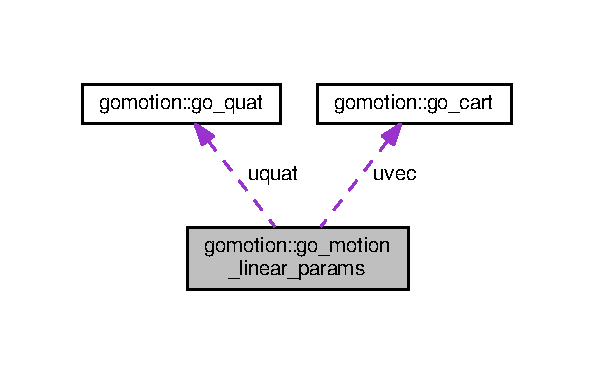
\includegraphics[width=285pt]{d6/dbf/structgomotion_1_1go__motion__linear__params__coll__graph}
\end{center}
\end{figure}
\subsection*{Data Fields}
\begin{DoxyCompactItemize}
\item 
\hyperlink{structgomotion_1_1go__cart}{go\-\_\-cart} \hyperlink{structgomotion_1_1go__motion__linear__params_ab1865f783998b55efb3c97f62e6a4f7d}{uvec}
\item 
\hyperlink{structgomotion_1_1go__quat}{go\-\_\-quat} \hyperlink{structgomotion_1_1go__motion__linear__params_af354e180468997cc31fca9f21a9bc325}{uquat}
\end{DoxyCompactItemize}


\subsection{Detailed Description}
In the following comments, L\-I\-N, C\-I\-R and A\-L\-L refer to linear moves, circular moves and both, respectively. 

If they are not in parens, e.\-g., A\-L\-L\-:, you need to provide them for that type of motion. If they are in parens, e.\-g., (C\-I\-R), they are computed for you. 

\subsection{Field Documentation}
\hypertarget{structgomotion_1_1go__motion__linear__params_af354e180468997cc31fca9f21a9bc325}{\index{gomotion\-::go\-\_\-motion\-\_\-linear\-\_\-params@{gomotion\-::go\-\_\-motion\-\_\-linear\-\_\-params}!uquat@{uquat}}
\index{uquat@{uquat}!gomotion::go_motion_linear_params@{gomotion\-::go\-\_\-motion\-\_\-linear\-\_\-params}}
\subsubsection[{uquat}]{\setlength{\rightskip}{0pt plus 5cm}{\bf go\-\_\-quat} gomotion\-::go\-\_\-motion\-\_\-linear\-\_\-params\-::uquat}}\label{structgomotion_1_1go__motion__linear__params_af354e180468997cc31fca9f21a9bc325}
\hypertarget{structgomotion_1_1go__motion__linear__params_ab1865f783998b55efb3c97f62e6a4f7d}{\index{gomotion\-::go\-\_\-motion\-\_\-linear\-\_\-params@{gomotion\-::go\-\_\-motion\-\_\-linear\-\_\-params}!uvec@{uvec}}
\index{uvec@{uvec}!gomotion::go_motion_linear_params@{gomotion\-::go\-\_\-motion\-\_\-linear\-\_\-params}}
\subsubsection[{uvec}]{\setlength{\rightskip}{0pt plus 5cm}{\bf go\-\_\-cart} gomotion\-::go\-\_\-motion\-\_\-linear\-\_\-params\-::uvec}}\label{structgomotion_1_1go__motion__linear__params_ab1865f783998b55efb3c97f62e6a4f7d}


The documentation for this struct was generated from the following file\-:\begin{DoxyCompactItemize}
\item 
/usr/local/michalos/nistfanuc\-\_\-ws/src/gomotion/include/gomotion/\hyperlink{gomotion_8h}{gomotion.\-h}\end{DoxyCompactItemize}

\hypertarget{structgomotion_1_1go__motion__params}{\section{gomotion\-:\-:go\-\_\-motion\-\_\-params Struct Reference}
\label{structgomotion_1_1go__motion__params}\index{gomotion\-::go\-\_\-motion\-\_\-params@{gomotion\-::go\-\_\-motion\-\_\-params}}
}


{\ttfamily \#include $<$gomotion.\-h$>$}

\subsection*{Data Fields}
\begin{DoxyCompactItemize}
\item 
\hyperlink{gotypes_8h_afd666a2393eebd71ee455846ac9def9b}{go\-\_\-real} \hyperlink{structgomotion_1_1go__motion__params_ad3121c36c5257557895df5d036b22c9d}{vel}
\begin{DoxyCompactList}\small\item\em max vel for each motion \end{DoxyCompactList}\item 
\hyperlink{gotypes_8h_afd666a2393eebd71ee455846ac9def9b}{go\-\_\-real} \hyperlink{structgomotion_1_1go__motion__params_a494815c0bc4016f78b82e2005ee6ad70}{acc}
\begin{DoxyCompactList}\small\item\em max accel for each motion \end{DoxyCompactList}\item 
\hyperlink{gotypes_8h_afd666a2393eebd71ee455846ac9def9b}{go\-\_\-real} \hyperlink{structgomotion_1_1go__motion__params_a25db76d9565efdc899bc8bc28b4a7c32}{jerk}
\begin{DoxyCompactList}\small\item\em max jerk for each motion \end{DoxyCompactList}\end{DoxyCompactItemize}


\subsection{Field Documentation}
\hypertarget{structgomotion_1_1go__motion__params_a494815c0bc4016f78b82e2005ee6ad70}{\index{gomotion\-::go\-\_\-motion\-\_\-params@{gomotion\-::go\-\_\-motion\-\_\-params}!acc@{acc}}
\index{acc@{acc}!gomotion::go_motion_params@{gomotion\-::go\-\_\-motion\-\_\-params}}
\subsubsection[{acc}]{\setlength{\rightskip}{0pt plus 5cm}{\bf go\-\_\-real} gomotion\-::go\-\_\-motion\-\_\-params\-::acc}}\label{structgomotion_1_1go__motion__params_a494815c0bc4016f78b82e2005ee6ad70}


max accel for each motion 

\hypertarget{structgomotion_1_1go__motion__params_a25db76d9565efdc899bc8bc28b4a7c32}{\index{gomotion\-::go\-\_\-motion\-\_\-params@{gomotion\-::go\-\_\-motion\-\_\-params}!jerk@{jerk}}
\index{jerk@{jerk}!gomotion::go_motion_params@{gomotion\-::go\-\_\-motion\-\_\-params}}
\subsubsection[{jerk}]{\setlength{\rightskip}{0pt plus 5cm}{\bf go\-\_\-real} gomotion\-::go\-\_\-motion\-\_\-params\-::jerk}}\label{structgomotion_1_1go__motion__params_a25db76d9565efdc899bc8bc28b4a7c32}


max jerk for each motion 

\hypertarget{structgomotion_1_1go__motion__params_ad3121c36c5257557895df5d036b22c9d}{\index{gomotion\-::go\-\_\-motion\-\_\-params@{gomotion\-::go\-\_\-motion\-\_\-params}!vel@{vel}}
\index{vel@{vel}!gomotion::go_motion_params@{gomotion\-::go\-\_\-motion\-\_\-params}}
\subsubsection[{vel}]{\setlength{\rightskip}{0pt plus 5cm}{\bf go\-\_\-real} gomotion\-::go\-\_\-motion\-\_\-params\-::vel}}\label{structgomotion_1_1go__motion__params_ad3121c36c5257557895df5d036b22c9d}


max vel for each motion 



The documentation for this struct was generated from the following file\-:\begin{DoxyCompactItemize}
\item 
/usr/local/michalos/nistfanuc\-\_\-ws/src/gomotion/include/gomotion/\hyperlink{gomotion_8h}{gomotion.\-h}\end{DoxyCompactItemize}

\hypertarget{structgomotion_1_1go__motion__queue}{\section{gomotion\-:\-:go\-\_\-motion\-\_\-queue Struct Reference}
\label{structgomotion_1_1go__motion__queue}\index{gomotion\-::go\-\_\-motion\-\_\-queue@{gomotion\-::go\-\_\-motion\-\_\-queue}}
}
\subsection*{Public Member Functions}
\begin{DoxyCompactItemize}
\item 
\hypertarget{structgomotion_1_1go__motion__queue_a23b5be5b838cf78eff17f8a7fa5df490}{go\-\_\-result {\bfseries init} (\hyperlink{structgomotion_1_1go__motion__spec}{go\-\_\-motion\-\_\-spec} $\ast$space, go\-\_\-integer size, go\-\_\-real deltat)}\label{structgomotion_1_1go__motion__queue_a23b5be5b838cf78eff17f8a7fa5df490}

\item 
go\-\_\-result \hyperlink{structgomotion_1_1go__motion__queue_a2eb9870461c0c071b2576c0071aebae7}{reset} ()
\begin{DoxyCompactList}\small\item\em Reset motion queue. Null motion type, reset start and set end to start, Zero number of motions on queue, last\-\_\-id of motion on queue, time. Init timescale to 1.\-0. \end{DoxyCompactList}\item 
go\-\_\-result \hyperlink{structgomotion_1_1go__motion__queue_a7ecc32334fd878989a9c1aba2dd8f309}{set\-\_\-type} (go\-\_\-flag type)
\begin{DoxyCompactList}\small\item\em Set type of motion queueing done\-: G\-O\-\_\-\-M\-O\-T\-I\-O\-N\-\_\-\-N\-O\-N\-E, G\-O\-\_\-\-M\-O\-T\-I\-O\-N\-\_\-\-J\-O\-I\-N\-T, G\-O\-\_\-\-M\-O\-T\-I\-O\-N\-\_\-\-U\-J\-O\-I\-N\-T, G\-O\-\_\-\-M\-O\-T\-I\-O\-N\-\_\-\-W\-O\-R\-L\-D. \end{DoxyCompactList}\item 
\hypertarget{structgomotion_1_1go__motion__queue_a29775f13e13d7ca216e416c87b14fcdb}{go\-\_\-flag {\bfseries get\-\_\-type} ()}\label{structgomotion_1_1go__motion__queue_a29775f13e13d7ca216e416c87b14fcdb}

\item 
go\-\_\-result \hyperlink{structgomotion_1_1go__motion__queue_ac623c003c01542bea2151f38b622c67e}{set\-\_\-joint\-\_\-number} (go\-\_\-integer joints)
\begin{DoxyCompactList}\small\item\em Set number of joints. Must positive andless than G\-O\-\_\-\-M\-O\-T\-I\-O\-N\-\_\-\-J\-O\-I\-N\-T\-\_\-\-N\-U\-M. \end{DoxyCompactList}\item 
go\-\_\-integer \hyperlink{structgomotion_1_1go__motion__queue_ac2fcc83c90ccd7794d7407174eaf2b37}{get\-\_\-joint\-\_\-number} ()
\begin{DoxyCompactList}\small\item\em Get number of joints. \end{DoxyCompactList}\item 
go\-\_\-result \hyperlink{structgomotion_1_1go__motion__queue_a0580645d22f2db0893ccd1cc0271469d}{set\-\_\-here} (const \hyperlink{structgomotion_1_1go__position}{go\-\_\-position} $\ast$\hyperlink{structgomotion_1_1go__motion__queue_ab45a3644aac5d496e758db38a3553037}{here})
\begin{DoxyCompactList}\small\item\em Set current position -\/ either joint values or world Cartesian pose. \end{DoxyCompactList}\item 
go\-\_\-result \hyperlink{structgomotion_1_1go__motion__queue_a560b24166fe53f8e2d8be6afaf08c7e9}{set\-\_\-cycle\-\_\-time} (go\-\_\-real deltat)
\begin{DoxyCompactList}\small\item\em Set deltat, the time in seconds per cycle. \end{DoxyCompactList}\item 
\hypertarget{structgomotion_1_1go__motion__queue_addfc802fee86a93050de27d185c4030b}{go\-\_\-result {\bfseries set\-\_\-scale} (go\-\_\-real scale, go\-\_\-real scale\-\_\-v, go\-\_\-real scale\-\_\-a)}\label{structgomotion_1_1go__motion__queue_addfc802fee86a93050de27d185c4030b}

\item 
go\-\_\-result \hyperlink{structgomotion_1_1go__motion__queue_aed6b10eacd99af71b2b0cf69d6ddebeb}{append} (const \hyperlink{structgomotion_1_1go__motion__spec}{go\-\_\-motion\-\_\-spec} $\ast$motion)
\begin{DoxyCompactList}\small\item\em Append motion\-\_\-spec onto queue. if type is G\-O\-\_\-\-M\-O\-T\-I\-O\-N\-\_\-\-J\-O\-I\-N\-T then motion is done as append\-\_\-joint if type is G\-O\-\_\-\-M\-O\-T\-I\-O\-N\-\_\-\-U\-J\-O\-I\-N\-T then motion is done as append\-\_\-ujoint if type is G\-O\-\_\-\-M\-O\-T\-I\-O\-N\-\_\-\-W\-O\-R\-L\-D then motion is done as append\-\_\-world. \end{DoxyCompactList}\item 
\hypertarget{structgomotion_1_1go__motion__queue_a8dfbc19656f2dfcf1e99c27e6a909c4d}{go\-\_\-result {\bfseries number} (go\-\_\-integer $\ast$number)}\label{structgomotion_1_1go__motion__queue_a8dfbc19656f2dfcf1e99c27e6a909c4d}

\item 
\hypertarget{structgomotion_1_1go__motion__queue_a9eb929528abd0d19d272110c67236dce}{go\-\_\-result {\bfseries size} (go\-\_\-integer $\ast$size)}\label{structgomotion_1_1go__motion__queue_a9eb929528abd0d19d272110c67236dce}

\item 
go\-\_\-result \hyperlink{structgomotion_1_1go__motion__queue_a3fe40223c4ad5a19b929b192d7cead64}{head} (\hyperlink{structgomotion_1_1go__motion__spec}{go\-\_\-motion\-\_\-spec} $\ast$motion)
\begin{DoxyCompactList}\small\item\em Get the head of the motion queue. \end{DoxyCompactList}\item 
go\-\_\-result \hyperlink{structgomotion_1_1go__motion__queue_ab45a3644aac5d496e758db38a3553037}{here} (\hyperlink{structgomotion_1_1go__position}{go\-\_\-position} $\ast$position)
\begin{DoxyCompactList}\small\item\em Get the here position and store into pointer to \hyperlink{structgomotion_1_1go__motion__spec}{go\-\_\-motion\-\_\-spec}. \end{DoxyCompactList}\item 
go\-\_\-result \hyperlink{structgomotion_1_1go__motion__queue_ad5de56ac17a7e86ea66627376b668bd2}{there} (\hyperlink{structgomotion_1_1go__position}{go\-\_\-position} $\ast$position)
\begin{DoxyCompactList}\small\item\em Get the there position and store into the motion pointer to \hyperlink{structgomotion_1_1go__motion__spec}{go\-\_\-motion\-\_\-spec}. \end{DoxyCompactList}\item 
go\-\_\-result \hyperlink{structgomotion_1_1go__motion__queue_a3cfb410e307b2bd3af0c64406364edfc}{interp} (\hyperlink{structgomotion_1_1go__position}{go\-\_\-position} $\ast$position)
\begin{DoxyCompactList}\small\item\em Do interpret cycle and store result into position pointer. Only if there's something on the queue do we want to increment the queue time. It was set to 0 when the queue was emptied, and will not be set to zero when the next move is appended. \end{DoxyCompactList}\item 
\hypertarget{structgomotion_1_1go__motion__queue_a59932f32a219889d188e2b4184b396c2}{go\-\_\-result {\bfseries stop} (\hyperlink{structgomotion_1_1go__motion__queue}{go\-\_\-motion\-\_\-queue} $\ast$queue)}\label{structgomotion_1_1go__motion__queue_a59932f32a219889d188e2b4184b396c2}

\item 
go\-\_\-result \hyperlink{structgomotion_1_1go__motion__queue_a10c28cd42c87403852354d8a26e11204}{set\-\_\-id} (go\-\_\-integer id)
\begin{DoxyCompactList}\small\item\em Set id of last motion appended. \end{DoxyCompactList}\item 
go\-\_\-integer \hyperlink{structgomotion_1_1go__motion__queue_ab6be3f8589b1ed1d0cf9615c16d3f7cd}{last\-\_\-id} ()
\begin{DoxyCompactList}\small\item\em Get id of last motion appended. \end{DoxyCompactList}\item 
\hypertarget{structgomotion_1_1go__motion__queue_ad159c5ff1a51e68707caf4c6466da2cb}{go\-\_\-flag {\bfseries is\-\_\-empty} ()}\label{structgomotion_1_1go__motion__queue_ad159c5ff1a51e68707caf4c6466da2cb}

\item 
\hypertarget{structgomotion_1_1go__motion__queue_a0f48a4983551ffa4d5e53e3c62a965c6}{go\-\_\-result {\bfseries erase} ()}\label{structgomotion_1_1go__motion__queue_a0f48a4983551ffa4d5e53e3c62a965c6}

\item 
\hypertarget{structgomotion_1_1go__motion__queue_ac14fbfab39c746da1969390c50617746}{go\-\_\-result {\bfseries drop\-\_\-pending} ()}\label{structgomotion_1_1go__motion__queue_ac14fbfab39c746da1969390c50617746}

\item 
go\-\_\-result \hyperlink{structgomotion_1_1go__motion__queue_ad2fa3a736879c90c0ffbdf7bc0bc54c9}{stop} ()
\begin{DoxyCompactList}\small\item\em Stop queue interpret cycle now. Don't need to stop an empty or stopping queue store computed joint/world motion. point our attention at the current motion. Call go\-\_\-traj\-\_\-cj\-\_\-stop for each joint-\/ or tran/rot motion, so that each stops as fast as it can. The longest to stop will set the revised stop time, and each will be extended to stop at that longest time. Note that the specptr values are incremental for the move, as the original distance passed to go\-\_\-traj\-\_\-cj\-\_\-compute was the incremental distance. \end{DoxyCompactList}\end{DoxyCompactItemize}
\subsection*{Protected Member Functions}
\begin{DoxyCompactItemize}
\item 
\hypertarget{structgomotion_1_1go__motion__queue_a8530405c3ab2eb49c99b78804af3110f}{go\-\_\-result {\bfseries append\-\_\-joint} (const \hyperlink{structgomotion_1_1go__motion__spec}{go\-\_\-motion\-\_\-spec} $\ast$motion)}\label{structgomotion_1_1go__motion__queue_a8530405c3ab2eb49c99b78804af3110f}

\item 
\hypertarget{structgomotion_1_1go__motion__queue_a9764d6dc903c426e1e5277bc2ffd26bc}{go\-\_\-result {\bfseries append\-\_\-ujoint} (const \hyperlink{structgomotion_1_1go__motion__spec}{go\-\_\-motion\-\_\-spec} $\ast$motion)}\label{structgomotion_1_1go__motion__queue_a9764d6dc903c426e1e5277bc2ffd26bc}

\item 
\hypertarget{structgomotion_1_1go__motion__queue_a59948ff83135837e9b87385a4b220571}{go\-\_\-result {\bfseries append\-\_\-world} (const \hyperlink{structgomotion_1_1go__motion__spec}{go\-\_\-motion\-\_\-spec} $\ast$motion)}\label{structgomotion_1_1go__motion__queue_a59948ff83135837e9b87385a4b220571}

\item 
\hypertarget{structgomotion_1_1go__motion__queue_a6d7f6a8773b64aa9dfa95639288634c6}{go\-\_\-result {\bfseries interp\-\_\-joint} (go\-\_\-real $\ast$joint)}\label{structgomotion_1_1go__motion__queue_a6d7f6a8773b64aa9dfa95639288634c6}

\item 
\hypertarget{structgomotion_1_1go__motion__queue_a992ce6f5b03fc13da0fbd438d9bdb625}{go\-\_\-result {\bfseries interp\-\_\-world} (go\-\_\-pose $\ast$pose)}\label{structgomotion_1_1go__motion__queue_a992ce6f5b03fc13da0fbd438d9bdb625}

\item 
\hypertarget{structgomotion_1_1go__motion__queue_a5b0db307f2635f1cf5b643f68aed98ab}{go\-\_\-result {\bfseries interp\-\_\-world} (\hyperlink{structgomotion_1_1go__motion__spec}{go\-\_\-motion\-\_\-spec} $\ast$motion, go\-\_\-real time, go\-\_\-pose $\ast$pose)}\label{structgomotion_1_1go__motion__queue_a5b0db307f2635f1cf5b643f68aed98ab}

\end{DoxyCompactItemize}
\subsection*{Protected Attributes}
\begin{DoxyCompactItemize}
\item 
go\-\_\-flag \hyperlink{structgomotion_1_1go__motion__queue_a0c5400b47c8a5e5966da98832ddad2dd}{\-\_\-type}
\item 
\hyperlink{structgomotion_1_1go__position}{go\-\_\-position} \hyperlink{structgomotion_1_1go__motion__queue_a9df9c96ad6bbcbb60c0c58754790d83b}{\-\_\-here}
\item 
\hyperlink{structgomotion_1_1go__position}{go\-\_\-position} \hyperlink{structgomotion_1_1go__motion__queue_a96ac4977f0e8c0a01930f945262015fa}{\-\_\-there}
\item 
\hyperlink{structgomotion_1_1go__motion__spec}{go\-\_\-motion\-\_\-spec} $\ast$ \hyperlink{structgomotion_1_1go__motion__queue_a0115449f0ee391d3e1d473e5861d594e}{\-\_\-startptr}
\item 
\hyperlink{structgomotion_1_1go__motion__spec}{go\-\_\-motion\-\_\-spec} $\ast$ \hyperlink{structgomotion_1_1go__motion__queue_a56b0eb35d9ff084d1a1f555dae780ad9}{\-\_\-endptr}
\item 
\hyperlink{structgomotion_1_1go__motion__spec}{go\-\_\-motion\-\_\-spec} $\ast$ \hyperlink{structgomotion_1_1go__motion__queue_aa48dfdfd799a6cf63856b760d264c23b}{\-\_\-start}
\item 
\hyperlink{structgomotion_1_1go__motion__spec}{go\-\_\-motion\-\_\-spec} $\ast$ \hyperlink{structgomotion_1_1go__motion__queue_a843d9fbbb3d45019e412efe56e3356a9}{\-\_\-end}
\item 
go\-\_\-integer \hyperlink{structgomotion_1_1go__motion__queue_adc9cde829948ecc241cdcaa5b839c888}{\-\_\-size}
\item 
go\-\_\-integer \hyperlink{structgomotion_1_1go__motion__queue_ab1ba219a6f370e7df6495ca0fd958108}{\-\_\-joint\-\_\-num}
\item 
go\-\_\-integer \hyperlink{structgomotion_1_1go__motion__queue_a1c1fe7f38ef5ba8523d251d2199a19e3}{\-\_\-number}
\item 
go\-\_\-integer \hyperlink{structgomotion_1_1go__motion__queue_aeba2a7bb2b6dd7076aed9cc51904f312}{\-\_\-last\-\_\-id}
\item 
go\-\_\-real \hyperlink{structgomotion_1_1go__motion__queue_a21be21caeb469dc31cae7e4d193f6f63}{\-\_\-deltat}
\item 
go\-\_\-real \hyperlink{structgomotion_1_1go__motion__queue_a9f72301ca7a9a96fde11f519c097cdaf}{\-\_\-time}
\item 
\hyperlink{structgomotion_1_1go__scale__spec}{go\-\_\-scale\-\_\-spec} \hyperlink{structgomotion_1_1go__motion__queue_a78ce1642f13b46e810ae781a827408e6}{\-\_\-timescale}
\end{DoxyCompactItemize}


\subsection{Member Function Documentation}
\hypertarget{structgomotion_1_1go__motion__queue_aed6b10eacd99af71b2b0cf69d6ddebeb}{\index{gomotion\-::go\-\_\-motion\-\_\-queue@{gomotion\-::go\-\_\-motion\-\_\-queue}!append@{append}}
\index{append@{append}!gomotion::go_motion_queue@{gomotion\-::go\-\_\-motion\-\_\-queue}}
\subsubsection[{append}]{\setlength{\rightskip}{0pt plus 5cm}go\-\_\-result gomotion\-::go\-\_\-motion\-\_\-queue\-::append (
\begin{DoxyParamCaption}
\item[{const {\bf go\-\_\-motion\-\_\-spec} $\ast$}]{motion}
\end{DoxyParamCaption}
)}}\label{structgomotion_1_1go__motion__queue_aed6b10eacd99af71b2b0cf69d6ddebeb}


Append motion\-\_\-spec onto queue. if type is G\-O\-\_\-\-M\-O\-T\-I\-O\-N\-\_\-\-J\-O\-I\-N\-T then motion is done as append\-\_\-joint if type is G\-O\-\_\-\-M\-O\-T\-I\-O\-N\-\_\-\-U\-J\-O\-I\-N\-T then motion is done as append\-\_\-ujoint if type is G\-O\-\_\-\-M\-O\-T\-I\-O\-N\-\_\-\-W\-O\-R\-L\-D then motion is done as append\-\_\-world. 


\begin{DoxyParams}{Parameters}
{\em motion} & is a pointer to a motion spec. \\
\hline
\end{DoxyParams}
\begin{DoxyReturn}{Returns}
go\-\_\-result success or failure 
\end{DoxyReturn}
\hypertarget{structgomotion_1_1go__motion__queue_ac2fcc83c90ccd7794d7407174eaf2b37}{\index{gomotion\-::go\-\_\-motion\-\_\-queue@{gomotion\-::go\-\_\-motion\-\_\-queue}!get\-\_\-joint\-\_\-number@{get\-\_\-joint\-\_\-number}}
\index{get\-\_\-joint\-\_\-number@{get\-\_\-joint\-\_\-number}!gomotion::go_motion_queue@{gomotion\-::go\-\_\-motion\-\_\-queue}}
\subsubsection[{get\-\_\-joint\-\_\-number}]{\setlength{\rightskip}{0pt plus 5cm}go\-\_\-integer gomotion\-::go\-\_\-motion\-\_\-queue\-::get\-\_\-joint\-\_\-number (
\begin{DoxyParamCaption}
{}
\end{DoxyParamCaption}
)}}\label{structgomotion_1_1go__motion__queue_ac2fcc83c90ccd7794d7407174eaf2b37}


Get number of joints. 

\begin{DoxyReturn}{Returns}
integer 
\end{DoxyReturn}
\hypertarget{structgomotion_1_1go__motion__queue_a3fe40223c4ad5a19b929b192d7cead64}{\index{gomotion\-::go\-\_\-motion\-\_\-queue@{gomotion\-::go\-\_\-motion\-\_\-queue}!head@{head}}
\index{head@{head}!gomotion::go_motion_queue@{gomotion\-::go\-\_\-motion\-\_\-queue}}
\subsubsection[{head}]{\setlength{\rightskip}{0pt plus 5cm}go\-\_\-result gomotion\-::go\-\_\-motion\-\_\-queue\-::head (
\begin{DoxyParamCaption}
\item[{{\bf go\-\_\-motion\-\_\-spec} $\ast$}]{motion}
\end{DoxyParamCaption}
)}}\label{structgomotion_1_1go__motion__queue_a3fe40223c4ad5a19b929b192d7cead64}


Get the head of the motion queue. 


\begin{DoxyParams}{Parameters}
{\em motion} & is a pointer to store the head of the motion queue. \\
\hline
\end{DoxyParams}
\begin{DoxyReturn}{Returns}
go\-\_\-result success or failure 
\end{DoxyReturn}
\hypertarget{structgomotion_1_1go__motion__queue_ab45a3644aac5d496e758db38a3553037}{\index{gomotion\-::go\-\_\-motion\-\_\-queue@{gomotion\-::go\-\_\-motion\-\_\-queue}!here@{here}}
\index{here@{here}!gomotion::go_motion_queue@{gomotion\-::go\-\_\-motion\-\_\-queue}}
\subsubsection[{here}]{\setlength{\rightskip}{0pt plus 5cm}go\-\_\-result gomotion\-::go\-\_\-motion\-\_\-queue\-::here (
\begin{DoxyParamCaption}
\item[{{\bf go\-\_\-position} $\ast$}]{position}
\end{DoxyParamCaption}
)}}\label{structgomotion_1_1go__motion__queue_ab45a3644aac5d496e758db38a3553037}


Get the here position and store into pointer to \hyperlink{structgomotion_1_1go__motion__spec}{go\-\_\-motion\-\_\-spec}. 


\begin{DoxyParams}{Parameters}
{\em position} & is a pointer to store here motion spec. \\
\hline
\end{DoxyParams}
\begin{DoxyReturn}{Returns}
go\-\_\-result success or failure 
\end{DoxyReturn}
\hypertarget{structgomotion_1_1go__motion__queue_a3cfb410e307b2bd3af0c64406364edfc}{\index{gomotion\-::go\-\_\-motion\-\_\-queue@{gomotion\-::go\-\_\-motion\-\_\-queue}!interp@{interp}}
\index{interp@{interp}!gomotion::go_motion_queue@{gomotion\-::go\-\_\-motion\-\_\-queue}}
\subsubsection[{interp}]{\setlength{\rightskip}{0pt plus 5cm}go\-\_\-result gomotion\-::go\-\_\-motion\-\_\-queue\-::interp (
\begin{DoxyParamCaption}
\item[{{\bf go\-\_\-position} $\ast$}]{position}
\end{DoxyParamCaption}
)}}\label{structgomotion_1_1go__motion__queue_a3cfb410e307b2bd3af0c64406364edfc}


Do interpret cycle and store result into position pointer. Only if there's something on the queue do we want to increment the queue time. It was set to 0 when the queue was emptied, and will not be set to zero when the next move is appended. 


\begin{DoxyParams}{Parameters}
{\em position} & is a pointer to store computed joint/world motion. \\
\hline
\end{DoxyParams}
\begin{DoxyReturn}{Returns}
go\-\_\-result success or failure 
\end{DoxyReturn}
\hypertarget{structgomotion_1_1go__motion__queue_ab6be3f8589b1ed1d0cf9615c16d3f7cd}{\index{gomotion\-::go\-\_\-motion\-\_\-queue@{gomotion\-::go\-\_\-motion\-\_\-queue}!last\-\_\-id@{last\-\_\-id}}
\index{last\-\_\-id@{last\-\_\-id}!gomotion::go_motion_queue@{gomotion\-::go\-\_\-motion\-\_\-queue}}
\subsubsection[{last\-\_\-id}]{\setlength{\rightskip}{0pt plus 5cm}go\-\_\-integer gomotion\-::go\-\_\-motion\-\_\-queue\-::last\-\_\-id (
\begin{DoxyParamCaption}
{}
\end{DoxyParamCaption}
)}}\label{structgomotion_1_1go__motion__queue_ab6be3f8589b1ed1d0cf9615c16d3f7cd}


Get id of last motion appended. 

\begin{DoxyReturn}{Returns}
integer value of motion. 
\end{DoxyReturn}
\hypertarget{structgomotion_1_1go__motion__queue_a2eb9870461c0c071b2576c0071aebae7}{\index{gomotion\-::go\-\_\-motion\-\_\-queue@{gomotion\-::go\-\_\-motion\-\_\-queue}!reset@{reset}}
\index{reset@{reset}!gomotion::go_motion_queue@{gomotion\-::go\-\_\-motion\-\_\-queue}}
\subsubsection[{reset}]{\setlength{\rightskip}{0pt plus 5cm}go\-\_\-result gomotion\-::go\-\_\-motion\-\_\-queue\-::reset (
\begin{DoxyParamCaption}
{}
\end{DoxyParamCaption}
)}}\label{structgomotion_1_1go__motion__queue_a2eb9870461c0c071b2576c0071aebae7}


Reset motion queue. Null motion type, reset start and set end to start, Zero number of motions on queue, last\-\_\-id of motion on queue, time. Init timescale to 1.\-0. 

\begin{DoxyReturn}{Returns}
go\-\_\-result success or failure 
\end{DoxyReturn}
\hypertarget{structgomotion_1_1go__motion__queue_a560b24166fe53f8e2d8be6afaf08c7e9}{\index{gomotion\-::go\-\_\-motion\-\_\-queue@{gomotion\-::go\-\_\-motion\-\_\-queue}!set\-\_\-cycle\-\_\-time@{set\-\_\-cycle\-\_\-time}}
\index{set\-\_\-cycle\-\_\-time@{set\-\_\-cycle\-\_\-time}!gomotion::go_motion_queue@{gomotion\-::go\-\_\-motion\-\_\-queue}}
\subsubsection[{set\-\_\-cycle\-\_\-time}]{\setlength{\rightskip}{0pt plus 5cm}go\-\_\-result gomotion\-::go\-\_\-motion\-\_\-queue\-::set\-\_\-cycle\-\_\-time (
\begin{DoxyParamCaption}
\item[{go\-\_\-real}]{deltat}
\end{DoxyParamCaption}
)}}\label{structgomotion_1_1go__motion__queue_a560b24166fe53f8e2d8be6afaf08c7e9}


Set deltat, the time in seconds per cycle. 


\begin{DoxyParams}{Parameters}
{\em deltat} & is time in real seconds, so fractional seconds possible. \\
\hline
\end{DoxyParams}
\begin{DoxyReturn}{Returns}
go\-\_\-result success or failure 
\end{DoxyReturn}
\hypertarget{structgomotion_1_1go__motion__queue_a0580645d22f2db0893ccd1cc0271469d}{\index{gomotion\-::go\-\_\-motion\-\_\-queue@{gomotion\-::go\-\_\-motion\-\_\-queue}!set\-\_\-here@{set\-\_\-here}}
\index{set\-\_\-here@{set\-\_\-here}!gomotion::go_motion_queue@{gomotion\-::go\-\_\-motion\-\_\-queue}}
\subsubsection[{set\-\_\-here}]{\setlength{\rightskip}{0pt plus 5cm}go\-\_\-result gomotion\-::go\-\_\-motion\-\_\-queue\-::set\-\_\-here (
\begin{DoxyParamCaption}
\item[{const {\bf go\-\_\-position} $\ast$}]{here}
\end{DoxyParamCaption}
)}}\label{structgomotion_1_1go__motion__queue_a0580645d22f2db0893ccd1cc0271469d}


Set current position -\/ either joint values or world Cartesian pose. 


\begin{DoxyParams}{Parameters}
{\em here} & as a pointer to a \hyperlink{structgomotion_1_1go__position}{go\-\_\-position} \\
\hline
\end{DoxyParams}
\begin{DoxyReturn}{Returns}
go\-\_\-result success or failure 
\end{DoxyReturn}
\hypertarget{structgomotion_1_1go__motion__queue_a10c28cd42c87403852354d8a26e11204}{\index{gomotion\-::go\-\_\-motion\-\_\-queue@{gomotion\-::go\-\_\-motion\-\_\-queue}!set\-\_\-id@{set\-\_\-id}}
\index{set\-\_\-id@{set\-\_\-id}!gomotion::go_motion_queue@{gomotion\-::go\-\_\-motion\-\_\-queue}}
\subsubsection[{set\-\_\-id}]{\setlength{\rightskip}{0pt plus 5cm}go\-\_\-result gomotion\-::go\-\_\-motion\-\_\-queue\-::set\-\_\-id (
\begin{DoxyParamCaption}
\item[{go\-\_\-integer}]{id}
\end{DoxyParamCaption}
)}}\label{structgomotion_1_1go__motion__queue_a10c28cd42c87403852354d8a26e11204}


Set id of last motion appended. 


\begin{DoxyParams}{Parameters}
{\em integer} & value for last id of motion queued. F\-I\-X\-M\-E\-: why would it ever not be incremental? \\
\hline
\end{DoxyParams}
\begin{DoxyReturn}{Returns}
go\-\_\-result success or failure 
\end{DoxyReturn}
\hypertarget{structgomotion_1_1go__motion__queue_ac623c003c01542bea2151f38b622c67e}{\index{gomotion\-::go\-\_\-motion\-\_\-queue@{gomotion\-::go\-\_\-motion\-\_\-queue}!set\-\_\-joint\-\_\-number@{set\-\_\-joint\-\_\-number}}
\index{set\-\_\-joint\-\_\-number@{set\-\_\-joint\-\_\-number}!gomotion::go_motion_queue@{gomotion\-::go\-\_\-motion\-\_\-queue}}
\subsubsection[{set\-\_\-joint\-\_\-number}]{\setlength{\rightskip}{0pt plus 5cm}go\-\_\-result gomotion\-::go\-\_\-motion\-\_\-queue\-::set\-\_\-joint\-\_\-number (
\begin{DoxyParamCaption}
\item[{go\-\_\-integer}]{joints}
\end{DoxyParamCaption}
)}}\label{structgomotion_1_1go__motion__queue_ac623c003c01542bea2151f38b622c67e}


Set number of joints. Must positive andless than G\-O\-\_\-\-M\-O\-T\-I\-O\-N\-\_\-\-J\-O\-I\-N\-T\-\_\-\-N\-U\-M. 


\begin{DoxyParams}{Parameters}
{\em joints} & number of joints \\
\hline
\end{DoxyParams}
\begin{DoxyReturn}{Returns}
go\-\_\-result success or failure 
\end{DoxyReturn}
\hypertarget{structgomotion_1_1go__motion__queue_a7ecc32334fd878989a9c1aba2dd8f309}{\index{gomotion\-::go\-\_\-motion\-\_\-queue@{gomotion\-::go\-\_\-motion\-\_\-queue}!set\-\_\-type@{set\-\_\-type}}
\index{set\-\_\-type@{set\-\_\-type}!gomotion::go_motion_queue@{gomotion\-::go\-\_\-motion\-\_\-queue}}
\subsubsection[{set\-\_\-type}]{\setlength{\rightskip}{0pt plus 5cm}go\-\_\-result gomotion\-::go\-\_\-motion\-\_\-queue\-::set\-\_\-type (
\begin{DoxyParamCaption}
\item[{go\-\_\-flag}]{type}
\end{DoxyParamCaption}
)}}\label{structgomotion_1_1go__motion__queue_a7ecc32334fd878989a9c1aba2dd8f309}


Set type of motion queueing done\-: G\-O\-\_\-\-M\-O\-T\-I\-O\-N\-\_\-\-N\-O\-N\-E, G\-O\-\_\-\-M\-O\-T\-I\-O\-N\-\_\-\-J\-O\-I\-N\-T, G\-O\-\_\-\-M\-O\-T\-I\-O\-N\-\_\-\-U\-J\-O\-I\-N\-T, G\-O\-\_\-\-M\-O\-T\-I\-O\-N\-\_\-\-W\-O\-R\-L\-D. 

these flags are used to further specify types of world motion\-: G\-O\-\_\-\-M\-O\-T\-I\-O\-N\-\_\-\-L\-I\-N\-E\-A\-R, G\-O\-\_\-\-M\-O\-T\-I\-O\-N\-\_\-\-C\-I\-R\-C\-U\-L\-A\-R \begin{DoxyReturn}{Returns}
go\-\_\-result success or failure 
\end{DoxyReturn}
\hypertarget{structgomotion_1_1go__motion__queue_ad2fa3a736879c90c0ffbdf7bc0bc54c9}{\index{gomotion\-::go\-\_\-motion\-\_\-queue@{gomotion\-::go\-\_\-motion\-\_\-queue}!stop@{stop}}
\index{stop@{stop}!gomotion::go_motion_queue@{gomotion\-::go\-\_\-motion\-\_\-queue}}
\subsubsection[{stop}]{\setlength{\rightskip}{0pt plus 5cm}go\-\_\-result gomotion\-::go\-\_\-motion\-\_\-queue\-::stop (
\begin{DoxyParamCaption}
{}
\end{DoxyParamCaption}
)}}\label{structgomotion_1_1go__motion__queue_ad2fa3a736879c90c0ffbdf7bc0bc54c9}


Stop queue interpret cycle now. Don't need to stop an empty or stopping queue store computed joint/world motion. point our attention at the current motion. Call go\-\_\-traj\-\_\-cj\-\_\-stop for each joint-\/ or tran/rot motion, so that each stops as fast as it can. The longest to stop will set the revised stop time, and each will be extended to stop at that longest time. Note that the specptr values are incremental for the move, as the original distance passed to go\-\_\-traj\-\_\-cj\-\_\-compute was the incremental distance. 

\begin{DoxyReturn}{Returns}
go\-\_\-result success or failure 
\end{DoxyReturn}
\hypertarget{structgomotion_1_1go__motion__queue_ad5de56ac17a7e86ea66627376b668bd2}{\index{gomotion\-::go\-\_\-motion\-\_\-queue@{gomotion\-::go\-\_\-motion\-\_\-queue}!there@{there}}
\index{there@{there}!gomotion::go_motion_queue@{gomotion\-::go\-\_\-motion\-\_\-queue}}
\subsubsection[{there}]{\setlength{\rightskip}{0pt plus 5cm}go\-\_\-result gomotion\-::go\-\_\-motion\-\_\-queue\-::there (
\begin{DoxyParamCaption}
\item[{{\bf go\-\_\-position} $\ast$}]{position}
\end{DoxyParamCaption}
)}}\label{structgomotion_1_1go__motion__queue_ad5de56ac17a7e86ea66627376b668bd2}


Get the there position and store into the motion pointer to \hyperlink{structgomotion_1_1go__motion__spec}{go\-\_\-motion\-\_\-spec}. 


\begin{DoxyParams}{Parameters}
{\em position} & is a pointer to store there motion spec. \\
\hline
\end{DoxyParams}
\begin{DoxyReturn}{Returns}
go\-\_\-result success or failure 
\end{DoxyReturn}


\subsection{Member Data Documentation}
\hypertarget{structgomotion_1_1go__motion__queue_a21be21caeb469dc31cae7e4d193f6f63}{\index{gomotion\-::go\-\_\-motion\-\_\-queue@{gomotion\-::go\-\_\-motion\-\_\-queue}!\-\_\-deltat@{\-\_\-deltat}}
\index{\-\_\-deltat@{\-\_\-deltat}!gomotion::go_motion_queue@{gomotion\-::go\-\_\-motion\-\_\-queue}}
\subsubsection[{\-\_\-deltat}]{\setlength{\rightskip}{0pt plus 5cm}go\-\_\-real gomotion\-::go\-\_\-motion\-\_\-queue\-::\-\_\-deltat\hspace{0.3cm}{\ttfamily [protected]}}}\label{structgomotion_1_1go__motion__queue_a21be21caeb469dc31cae7e4d193f6f63}
cycle time \hypertarget{structgomotion_1_1go__motion__queue_a843d9fbbb3d45019e412efe56e3356a9}{\index{gomotion\-::go\-\_\-motion\-\_\-queue@{gomotion\-::go\-\_\-motion\-\_\-queue}!\-\_\-end@{\-\_\-end}}
\index{\-\_\-end@{\-\_\-end}!gomotion::go_motion_queue@{gomotion\-::go\-\_\-motion\-\_\-queue}}
\subsubsection[{\-\_\-end}]{\setlength{\rightskip}{0pt plus 5cm}{\bf go\-\_\-motion\-\_\-spec}$\ast$ gomotion\-::go\-\_\-motion\-\_\-queue\-::\-\_\-end\hspace{0.3cm}{\ttfamily [protected]}}}\label{structgomotion_1_1go__motion__queue_a843d9fbbb3d45019e412efe56e3356a9}
ptr to last (empty) entry \hypertarget{structgomotion_1_1go__motion__queue_a56b0eb35d9ff084d1a1f555dae780ad9}{\index{gomotion\-::go\-\_\-motion\-\_\-queue@{gomotion\-::go\-\_\-motion\-\_\-queue}!\-\_\-endptr@{\-\_\-endptr}}
\index{\-\_\-endptr@{\-\_\-endptr}!gomotion::go_motion_queue@{gomotion\-::go\-\_\-motion\-\_\-queue}}
\subsubsection[{\-\_\-endptr}]{\setlength{\rightskip}{0pt plus 5cm}{\bf go\-\_\-motion\-\_\-spec}$\ast$ gomotion\-::go\-\_\-motion\-\_\-queue\-::\-\_\-endptr\hspace{0.3cm}{\ttfamily [protected]}}}\label{structgomotion_1_1go__motion__queue_a56b0eb35d9ff084d1a1f555dae780ad9}
the original end \hypertarget{structgomotion_1_1go__motion__queue_a9df9c96ad6bbcbb60c0c58754790d83b}{\index{gomotion\-::go\-\_\-motion\-\_\-queue@{gomotion\-::go\-\_\-motion\-\_\-queue}!\-\_\-here@{\-\_\-here}}
\index{\-\_\-here@{\-\_\-here}!gomotion::go_motion_queue@{gomotion\-::go\-\_\-motion\-\_\-queue}}
\subsubsection[{\-\_\-here}]{\setlength{\rightskip}{0pt plus 5cm}{\bf go\-\_\-position} gomotion\-::go\-\_\-motion\-\_\-queue\-::\-\_\-here\hspace{0.3cm}{\ttfamily [protected]}}}\label{structgomotion_1_1go__motion__queue_a9df9c96ad6bbcbb60c0c58754790d83b}
initial starting point \hypertarget{structgomotion_1_1go__motion__queue_ab1ba219a6f370e7df6495ca0fd958108}{\index{gomotion\-::go\-\_\-motion\-\_\-queue@{gomotion\-::go\-\_\-motion\-\_\-queue}!\-\_\-joint\-\_\-num@{\-\_\-joint\-\_\-num}}
\index{\-\_\-joint\-\_\-num@{\-\_\-joint\-\_\-num}!gomotion::go_motion_queue@{gomotion\-::go\-\_\-motion\-\_\-queue}}
\subsubsection[{\-\_\-joint\-\_\-num}]{\setlength{\rightskip}{0pt plus 5cm}go\-\_\-integer gomotion\-::go\-\_\-motion\-\_\-queue\-::\-\_\-joint\-\_\-num\hspace{0.3cm}{\ttfamily [protected]}}}\label{structgomotion_1_1go__motion__queue_ab1ba219a6f370e7df6495ca0fd958108}
number of joints to be interpolated \hypertarget{structgomotion_1_1go__motion__queue_aeba2a7bb2b6dd7076aed9cc51904f312}{\index{gomotion\-::go\-\_\-motion\-\_\-queue@{gomotion\-::go\-\_\-motion\-\_\-queue}!\-\_\-last\-\_\-id@{\-\_\-last\-\_\-id}}
\index{\-\_\-last\-\_\-id@{\-\_\-last\-\_\-id}!gomotion::go_motion_queue@{gomotion\-::go\-\_\-motion\-\_\-queue}}
\subsubsection[{\-\_\-last\-\_\-id}]{\setlength{\rightskip}{0pt plus 5cm}go\-\_\-integer gomotion\-::go\-\_\-motion\-\_\-queue\-::\-\_\-last\-\_\-id\hspace{0.3cm}{\ttfamily [protected]}}}\label{structgomotion_1_1go__motion__queue_aeba2a7bb2b6dd7076aed9cc51904f312}
id of last motion appended \hypertarget{structgomotion_1_1go__motion__queue_a1c1fe7f38ef5ba8523d251d2199a19e3}{\index{gomotion\-::go\-\_\-motion\-\_\-queue@{gomotion\-::go\-\_\-motion\-\_\-queue}!\-\_\-number@{\-\_\-number}}
\index{\-\_\-number@{\-\_\-number}!gomotion::go_motion_queue@{gomotion\-::go\-\_\-motion\-\_\-queue}}
\subsubsection[{\-\_\-number}]{\setlength{\rightskip}{0pt plus 5cm}go\-\_\-integer gomotion\-::go\-\_\-motion\-\_\-queue\-::\-\_\-number\hspace{0.3cm}{\ttfamily [protected]}}}\label{structgomotion_1_1go__motion__queue_a1c1fe7f38ef5ba8523d251d2199a19e3}
number of motions on queue \hypertarget{structgomotion_1_1go__motion__queue_adc9cde829948ecc241cdcaa5b839c888}{\index{gomotion\-::go\-\_\-motion\-\_\-queue@{gomotion\-::go\-\_\-motion\-\_\-queue}!\-\_\-size@{\-\_\-size}}
\index{\-\_\-size@{\-\_\-size}!gomotion::go_motion_queue@{gomotion\-::go\-\_\-motion\-\_\-queue}}
\subsubsection[{\-\_\-size}]{\setlength{\rightskip}{0pt plus 5cm}go\-\_\-integer gomotion\-::go\-\_\-motion\-\_\-queue\-::\-\_\-size\hspace{0.3cm}{\ttfamily [protected]}}}\label{structgomotion_1_1go__motion__queue_adc9cde829948ecc241cdcaa5b839c888}
size of whole queue \hypertarget{structgomotion_1_1go__motion__queue_aa48dfdfd799a6cf63856b760d264c23b}{\index{gomotion\-::go\-\_\-motion\-\_\-queue@{gomotion\-::go\-\_\-motion\-\_\-queue}!\-\_\-start@{\-\_\-start}}
\index{\-\_\-start@{\-\_\-start}!gomotion::go_motion_queue@{gomotion\-::go\-\_\-motion\-\_\-queue}}
\subsubsection[{\-\_\-start}]{\setlength{\rightskip}{0pt plus 5cm}{\bf go\-\_\-motion\-\_\-spec}$\ast$ gomotion\-::go\-\_\-motion\-\_\-queue\-::\-\_\-start\hspace{0.3cm}{\ttfamily [protected]}}}\label{structgomotion_1_1go__motion__queue_aa48dfdfd799a6cf63856b760d264c23b}
ptr to first entry of the queue \hypertarget{structgomotion_1_1go__motion__queue_a0115449f0ee391d3e1d473e5861d594e}{\index{gomotion\-::go\-\_\-motion\-\_\-queue@{gomotion\-::go\-\_\-motion\-\_\-queue}!\-\_\-startptr@{\-\_\-startptr}}
\index{\-\_\-startptr@{\-\_\-startptr}!gomotion::go_motion_queue@{gomotion\-::go\-\_\-motion\-\_\-queue}}
\subsubsection[{\-\_\-startptr}]{\setlength{\rightskip}{0pt plus 5cm}{\bf go\-\_\-motion\-\_\-spec}$\ast$ gomotion\-::go\-\_\-motion\-\_\-queue\-::\-\_\-startptr\hspace{0.3cm}{\ttfamily [protected]}}}\label{structgomotion_1_1go__motion__queue_a0115449f0ee391d3e1d473e5861d594e}
ptr to original start \hypertarget{structgomotion_1_1go__motion__queue_a96ac4977f0e8c0a01930f945262015fa}{\index{gomotion\-::go\-\_\-motion\-\_\-queue@{gomotion\-::go\-\_\-motion\-\_\-queue}!\-\_\-there@{\-\_\-there}}
\index{\-\_\-there@{\-\_\-there}!gomotion::go_motion_queue@{gomotion\-::go\-\_\-motion\-\_\-queue}}
\subsubsection[{\-\_\-there}]{\setlength{\rightskip}{0pt plus 5cm}{\bf go\-\_\-position} gomotion\-::go\-\_\-motion\-\_\-queue\-::\-\_\-there\hspace{0.3cm}{\ttfamily [protected]}}}\label{structgomotion_1_1go__motion__queue_a96ac4977f0e8c0a01930f945262015fa}
where the end is \hypertarget{structgomotion_1_1go__motion__queue_a9f72301ca7a9a96fde11f519c097cdaf}{\index{gomotion\-::go\-\_\-motion\-\_\-queue@{gomotion\-::go\-\_\-motion\-\_\-queue}!\-\_\-time@{\-\_\-time}}
\index{\-\_\-time@{\-\_\-time}!gomotion::go_motion_queue@{gomotion\-::go\-\_\-motion\-\_\-queue}}
\subsubsection[{\-\_\-time}]{\setlength{\rightskip}{0pt plus 5cm}go\-\_\-real gomotion\-::go\-\_\-motion\-\_\-queue\-::\-\_\-time\hspace{0.3cm}{\ttfamily [protected]}}}\label{structgomotion_1_1go__motion__queue_a9f72301ca7a9a96fde11f519c097cdaf}
time into the current spec \hypertarget{structgomotion_1_1go__motion__queue_a78ce1642f13b46e810ae781a827408e6}{\index{gomotion\-::go\-\_\-motion\-\_\-queue@{gomotion\-::go\-\_\-motion\-\_\-queue}!\-\_\-timescale@{\-\_\-timescale}}
\index{\-\_\-timescale@{\-\_\-timescale}!gomotion::go_motion_queue@{gomotion\-::go\-\_\-motion\-\_\-queue}}
\subsubsection[{\-\_\-timescale}]{\setlength{\rightskip}{0pt plus 5cm}{\bf go\-\_\-scale\-\_\-spec} gomotion\-::go\-\_\-motion\-\_\-queue\-::\-\_\-timescale\hspace{0.3cm}{\ttfamily [protected]}}}\label{structgomotion_1_1go__motion__queue_a78ce1642f13b46e810ae781a827408e6}
walked-\/in time scale factor \hypertarget{structgomotion_1_1go__motion__queue_a0c5400b47c8a5e5966da98832ddad2dd}{\index{gomotion\-::go\-\_\-motion\-\_\-queue@{gomotion\-::go\-\_\-motion\-\_\-queue}!\-\_\-type@{\-\_\-type}}
\index{\-\_\-type@{\-\_\-type}!gomotion::go_motion_queue@{gomotion\-::go\-\_\-motion\-\_\-queue}}
\subsubsection[{\-\_\-type}]{\setlength{\rightskip}{0pt plus 5cm}go\-\_\-flag gomotion\-::go\-\_\-motion\-\_\-queue\-::\-\_\-type\hspace{0.3cm}{\ttfamily [protected]}}}\label{structgomotion_1_1go__motion__queue_a0c5400b47c8a5e5966da98832ddad2dd}
go\-\_\-\-M\-O\-T\-I\-O\-N\-\_\-\-J\-O\-I\-N\-T for joint, otherwise world 

The documentation for this struct was generated from the following file\-:\begin{DoxyCompactItemize}
\item 
/usr/local/michalos/nistfanuc\-\_\-ws/src/gomotion/include/gomotion/\hyperlink{gomotion_8h}{gomotion.\-h}\end{DoxyCompactItemize}

\hypertarget{structgomotion_1_1go__motion__spec}{\section{gomotion\-:\-:go\-\_\-motion\-\_\-spec Struct Reference}
\label{structgomotion_1_1go__motion__spec}\index{gomotion\-::go\-\_\-motion\-\_\-spec@{gomotion\-::go\-\_\-motion\-\_\-spec}}
}
\subsection*{Public Member Functions}
\begin{DoxyCompactItemize}
\item 
go\-\_\-result \hyperlink{structgomotion_1_1go__motion__spec_a8a2282df2425f0eb1f258d1d0fadff5a}{init} ()
\begin{DoxyCompactList}\small\item\em Init the gomotion specification. If 'totalt' is positive, then it is the time for the move. Otherwise, it's automatically computed from the vel, acc and jerk, the usual case. Here we set 'totalt' to zero to get the usual case. \end{DoxyCompactList}\item 
go\-\_\-result \hyperlink{structgomotion_1_1go__motion__spec_a65efbbc70caff991679bbdd49fc9ccb9}{set\-\_\-type} (go\-\_\-flag \hyperlink{structgomotion_1_1go__motion__spec_a186231a66a1f1f6d6628cd23baf60530}{type})
\item 
\hypertarget{structgomotion_1_1go__motion__spec_a2d7aaadc8a968d43b563d83ad4d52cb3}{go\-\_\-flag {\bfseries get\-\_\-type} ()}\label{structgomotion_1_1go__motion__spec_a2d7aaadc8a968d43b563d83ad4d52cb3}

\item 
\hypertarget{structgomotion_1_1go__motion__spec_af5bd0446eb32dd4dfe9ae8811f820909}{go\-\_\-result {\bfseries set\-\_\-id} (go\-\_\-integer \hyperlink{structgomotion_1_1go__motion__spec_a09732ca7aaddfa7a637f171766329931}{id})}\label{structgomotion_1_1go__motion__spec_af5bd0446eb32dd4dfe9ae8811f820909}

\item 
\hypertarget{structgomotion_1_1go__motion__spec_a2ed1b68537a42747a67507eba4757b4f}{go\-\_\-integer {\bfseries get\-\_\-id} ()}\label{structgomotion_1_1go__motion__spec_a2ed1b68537a42747a67507eba4757b4f}

\item 
go\-\_\-result \hyperlink{structgomotion_1_1go__motion__spec_a5871885be899af7b09a7ec0f12945ece}{set\-\_\-jpar} (go\-\_\-integer i, go\-\_\-real vel, go\-\_\-real acc, go\-\_\-real jerk)
\begin{DoxyCompactList}\small\item\em Set a joint parameters. \end{DoxyCompactList}\item 
go\-\_\-result \hyperlink{structgomotion_1_1go__motion__spec_a31bdbdc08c0f922214a9c53d7dbc37ae}{set\-\_\-tpar} (go\-\_\-real vel, go\-\_\-real acc, go\-\_\-real jerk)
\begin{DoxyCompactList}\small\item\em Set world Cartesian translation parameters. \end{DoxyCompactList}\item 
go\-\_\-result \hyperlink{structgomotion_1_1go__motion__spec_a162ebe0197582af6807b88070dc3fd80}{set\-\_\-rpar} (go\-\_\-real vel, go\-\_\-real acc, go\-\_\-real jerk)
\begin{DoxyCompactList}\small\item\em Set world Cartesian rotational parameters. \end{DoxyCompactList}\item 
\hypertarget{structgomotion_1_1go__motion__spec_a64789307eff349e4fba3e93d301c0f49}{go\-\_\-result \hyperlink{structgomotion_1_1go__motion__spec_a64789307eff349e4fba3e93d301c0f49}{set\-\_\-cpar} (go\-\_\-cart $\ast$center, go\-\_\-cart $\ast$normal, go\-\_\-integer turns)}\label{structgomotion_1_1go__motion__spec_a64789307eff349e4fba3e93d301c0f49}

\begin{DoxyCompactList}\small\item\em Set circular rotation Cartesian move parameters. \end{DoxyCompactList}\item 
go\-\_\-result \hyperlink{structgomotion_1_1go__motion__spec_aad2d4b504cd2b02b1202bac4c134b7e9}{set\-\_\-time} (go\-\_\-real time)
\begin{DoxyCompactList}\small\item\em Set time to positive real number. \end{DoxyCompactList}\item 
go\-\_\-result \hyperlink{structgomotion_1_1go__motion__spec_ab71360b76432e6f584d09dc8c014971b}{set\-\_\-end\-\_\-position} (\hyperlink{structgomotion_1_1go__position}{go\-\_\-position} $\ast$\hyperlink{structgomotion_1_1go__motion__spec_a8e19d2d27bfa3a3c633bae73641f4e45}{end})
\begin{DoxyCompactList}\small\item\em If you are doing joint interpolation (as specified by your call to go\-\_\-motion\-\_\-queue\-\_\-set\-\_\-type()), et\-\_\-end\-\_\-position fills in joint\mbox{[}\mbox{]} accordingly. \end{DoxyCompactList}\item 
go\-\_\-result \hyperlink{structgomotion_1_1go__motion__spec_a611ec60ffee7577165ece8272cddd67a}{set\-\_\-end\-\_\-pose} (go\-\_\-pose $\ast$\hyperlink{structgomotion_1_1go__motion__spec_a8e19d2d27bfa3a3c633bae73641f4e45}{end})
\begin{DoxyCompactList}\small\item\em If you are doing world coordinate interpolation (as specified by your call to go\-\_\-motion\-\_\-queue\-\_\-set\-\_\-type()), set\-\_\-end\-\_\-position fills in ending pose accordingly. \end{DoxyCompactList}\end{DoxyCompactItemize}
\subsection*{Public Attributes}
\begin{DoxyCompactItemize}
\item 
go\-\_\-flag \hyperlink{structgomotion_1_1go__motion__spec_a186231a66a1f1f6d6628cd23baf60530}{type}
\item 
go\-\_\-integer \hyperlink{structgomotion_1_1go__motion__spec_a09732ca7aaddfa7a637f171766329931}{id}
\item 
go\-\_\-real \hyperlink{structgomotion_1_1go__motion__spec_abf6e879f2b06d62fe0bec48b9d723186}{totalt}
\item 
\hyperlink{structgomotion_1_1go__position}{go\-\_\-position} \hyperlink{structgomotion_1_1go__motion__spec_a87e745675e617e11ea1783a6ea80afa0}{start}
\item 
\hyperlink{structgomotion_1_1go__position}{go\-\_\-position} \hyperlink{structgomotion_1_1go__motion__spec_a8e19d2d27bfa3a3c633bae73641f4e45}{end}
\item 
go\-\_\-quat \hyperlink{structgomotion_1_1go__motion__spec_af21779ad35fe55e85d91bf8e133def52}{uquat}
\item 
\hyperlink{structgomotion_1_1go__motion__params}{go\-\_\-motion\-\_\-params} \hyperlink{structgomotion_1_1go__motion__spec_a71e60787cb50243693e8588918b8fe29}{par} \mbox{[}G\-O\-\_\-\-M\-O\-T\-I\-O\-N\-\_\-\-J\-O\-I\-N\-T\-\_\-\-N\-U\-M\mbox{]}
\item 
\hypertarget{structgomotion_1_1go__motion__spec_a259572286e5486f7b15870dc32988b74}{\begin{tabbing}
xx\=xx\=xx\=xx\=xx\=xx\=xx\=xx\=xx\=\kill
union \{\\
\>\hyperlink{structgomotion_1_1go__motion__linear__params}{go\_motion\_linear\_params} \hyperlink{structgomotion_1_1go__motion__spec_a25d35e4638e0dd5721409d02e2f48445}{lpar}\\
\>\hyperlink{structgomotion_1_1go__motion__circular__params}{go\_motion\_circular\_params} \hyperlink{structgomotion_1_1go__motion__spec_a4f8c8e620396ab92594d65f1d98bbdcc}{cpar}\\
\} {\bfseries u}}\label{structgomotion_1_1go__motion__spec_a259572286e5486f7b15870dc32988b74}
\\

\end{tabbing}\item 
\hypertarget{structgomotion_1_1go__motion__spec_ac585087da484a433071bfa02e712a979}{go\-\_\-traj\-\_\-cj\-\_\-spec {\bfseries cj} \mbox{[}G\-O\-\_\-\-M\-O\-T\-I\-O\-N\-\_\-\-J\-O\-I\-N\-T\-\_\-\-N\-U\-M\mbox{]}}\label{structgomotion_1_1go__motion__spec_ac585087da484a433071bfa02e712a979}

\end{DoxyCompactItemize}


\subsection{Member Function Documentation}
\hypertarget{structgomotion_1_1go__motion__spec_a8a2282df2425f0eb1f258d1d0fadff5a}{\index{gomotion\-::go\-\_\-motion\-\_\-spec@{gomotion\-::go\-\_\-motion\-\_\-spec}!init@{init}}
\index{init@{init}!gomotion::go_motion_spec@{gomotion\-::go\-\_\-motion\-\_\-spec}}
\subsubsection[{init}]{\setlength{\rightskip}{0pt plus 5cm}go\-\_\-result gomotion\-::go\-\_\-motion\-\_\-spec\-::init (
\begin{DoxyParamCaption}
{}
\end{DoxyParamCaption}
)}}\label{structgomotion_1_1go__motion__spec_a8a2282df2425f0eb1f258d1d0fadff5a}


Init the gomotion specification. If 'totalt' is positive, then it is the time for the move. Otherwise, it's automatically computed from the vel, acc and jerk, the usual case. Here we set 'totalt' to zero to get the usual case. 

\begin{DoxyReturn}{Returns}
go\-\_\-result success or failure 
\end{DoxyReturn}
\hypertarget{structgomotion_1_1go__motion__spec_a611ec60ffee7577165ece8272cddd67a}{\index{gomotion\-::go\-\_\-motion\-\_\-spec@{gomotion\-::go\-\_\-motion\-\_\-spec}!set\-\_\-end\-\_\-pose@{set\-\_\-end\-\_\-pose}}
\index{set\-\_\-end\-\_\-pose@{set\-\_\-end\-\_\-pose}!gomotion::go_motion_spec@{gomotion\-::go\-\_\-motion\-\_\-spec}}
\subsubsection[{set\-\_\-end\-\_\-pose}]{\setlength{\rightskip}{0pt plus 5cm}go\-\_\-result gomotion\-::go\-\_\-motion\-\_\-spec\-::set\-\_\-end\-\_\-pose (
\begin{DoxyParamCaption}
\item[{go\-\_\-pose $\ast$}]{end}
\end{DoxyParamCaption}
)}}\label{structgomotion_1_1go__motion__spec_a611ec60ffee7577165ece8272cddd67a}


If you are doing world coordinate interpolation (as specified by your call to go\-\_\-motion\-\_\-queue\-\_\-set\-\_\-type()), set\-\_\-end\-\_\-position fills in ending pose accordingly. 


\begin{DoxyParams}{Parameters}
{\em end} & is the end pose of the robot (position and orientation) \\
\hline
\end{DoxyParams}
\begin{DoxyReturn}{Returns}
go\-\_\-result success or failure 
\end{DoxyReturn}
\hypertarget{structgomotion_1_1go__motion__spec_ab71360b76432e6f584d09dc8c014971b}{\index{gomotion\-::go\-\_\-motion\-\_\-spec@{gomotion\-::go\-\_\-motion\-\_\-spec}!set\-\_\-end\-\_\-position@{set\-\_\-end\-\_\-position}}
\index{set\-\_\-end\-\_\-position@{set\-\_\-end\-\_\-position}!gomotion::go_motion_spec@{gomotion\-::go\-\_\-motion\-\_\-spec}}
\subsubsection[{set\-\_\-end\-\_\-position}]{\setlength{\rightskip}{0pt plus 5cm}go\-\_\-result gomotion\-::go\-\_\-motion\-\_\-spec\-::set\-\_\-end\-\_\-position (
\begin{DoxyParamCaption}
\item[{{\bf go\-\_\-position} $\ast$}]{end}
\end{DoxyParamCaption}
)}}\label{structgomotion_1_1go__motion__spec_ab71360b76432e6f584d09dc8c014971b}


If you are doing joint interpolation (as specified by your call to go\-\_\-motion\-\_\-queue\-\_\-set\-\_\-type()), et\-\_\-end\-\_\-position fills in joint\mbox{[}\mbox{]} accordingly. 


\begin{DoxyParams}{Parameters}
{\em end} & is the end position of the joints \\
\hline
\end{DoxyParams}
\begin{DoxyReturn}{Returns}
go\-\_\-result success or failure 
\end{DoxyReturn}
\hypertarget{structgomotion_1_1go__motion__spec_a5871885be899af7b09a7ec0f12945ece}{\index{gomotion\-::go\-\_\-motion\-\_\-spec@{gomotion\-::go\-\_\-motion\-\_\-spec}!set\-\_\-jpar@{set\-\_\-jpar}}
\index{set\-\_\-jpar@{set\-\_\-jpar}!gomotion::go_motion_spec@{gomotion\-::go\-\_\-motion\-\_\-spec}}
\subsubsection[{set\-\_\-jpar}]{\setlength{\rightskip}{0pt plus 5cm}go\-\_\-result gomotion\-::go\-\_\-motion\-\_\-spec\-::set\-\_\-jpar (
\begin{DoxyParamCaption}
\item[{go\-\_\-integer}]{i, }
\item[{go\-\_\-real}]{vel, }
\item[{go\-\_\-real}]{acc, }
\item[{go\-\_\-real}]{jerk}
\end{DoxyParamCaption}
)}}\label{structgomotion_1_1go__motion__spec_a5871885be899af7b09a7ec0f12945ece}


Set a joint parameters. 


\begin{DoxyParams}{Parameters}
{\em i} & joint number. \\
\hline
{\em vel} & velocity limit U\-N\-I\-T\-S? \\
\hline
{\em acc} & acceleration limit U\-N\-I\-T\-S? \\
\hline
{\em jerk} & jerk limit U\-N\-I\-T\-S? \\
\hline
\end{DoxyParams}
\begin{DoxyReturn}{Returns}
go\-\_\-result success or failure 
\end{DoxyReturn}
\hypertarget{structgomotion_1_1go__motion__spec_a162ebe0197582af6807b88070dc3fd80}{\index{gomotion\-::go\-\_\-motion\-\_\-spec@{gomotion\-::go\-\_\-motion\-\_\-spec}!set\-\_\-rpar@{set\-\_\-rpar}}
\index{set\-\_\-rpar@{set\-\_\-rpar}!gomotion::go_motion_spec@{gomotion\-::go\-\_\-motion\-\_\-spec}}
\subsubsection[{set\-\_\-rpar}]{\setlength{\rightskip}{0pt plus 5cm}go\-\_\-result gomotion\-::go\-\_\-motion\-\_\-spec\-::set\-\_\-rpar (
\begin{DoxyParamCaption}
\item[{go\-\_\-real}]{vel, }
\item[{go\-\_\-real}]{acc, }
\item[{go\-\_\-real}]{jerk}
\end{DoxyParamCaption}
)}}\label{structgomotion_1_1go__motion__spec_a162ebe0197582af6807b88070dc3fd80}


Set world Cartesian rotational parameters. 


\begin{DoxyParams}{Parameters}
{\em vel} & velocity limit U\-N\-I\-T\-S? \\
\hline
{\em acc} & acceleration limit U\-N\-I\-T\-S? \\
\hline
{\em jerk} & jerk limit U\-N\-I\-T\-S? \\
\hline
\end{DoxyParams}
\begin{DoxyReturn}{Returns}
go\-\_\-result success or failure 
\end{DoxyReturn}
\hypertarget{structgomotion_1_1go__motion__spec_aad2d4b504cd2b02b1202bac4c134b7e9}{\index{gomotion\-::go\-\_\-motion\-\_\-spec@{gomotion\-::go\-\_\-motion\-\_\-spec}!set\-\_\-time@{set\-\_\-time}}
\index{set\-\_\-time@{set\-\_\-time}!gomotion::go_motion_spec@{gomotion\-::go\-\_\-motion\-\_\-spec}}
\subsubsection[{set\-\_\-time}]{\setlength{\rightskip}{0pt plus 5cm}go\-\_\-result gomotion\-::go\-\_\-motion\-\_\-spec\-::set\-\_\-time (
\begin{DoxyParamCaption}
\item[{go\-\_\-real}]{time}
\end{DoxyParamCaption}
)}}\label{structgomotion_1_1go__motion__spec_aad2d4b504cd2b02b1202bac4c134b7e9}


Set time to positive real number. 


\begin{DoxyParams}{Parameters}
{\em time} & in seconds. \\
\hline
\end{DoxyParams}
\begin{DoxyReturn}{Returns}
go\-\_\-result success or failure 
\end{DoxyReturn}
\hypertarget{structgomotion_1_1go__motion__spec_a31bdbdc08c0f922214a9c53d7dbc37ae}{\index{gomotion\-::go\-\_\-motion\-\_\-spec@{gomotion\-::go\-\_\-motion\-\_\-spec}!set\-\_\-tpar@{set\-\_\-tpar}}
\index{set\-\_\-tpar@{set\-\_\-tpar}!gomotion::go_motion_spec@{gomotion\-::go\-\_\-motion\-\_\-spec}}
\subsubsection[{set\-\_\-tpar}]{\setlength{\rightskip}{0pt plus 5cm}go\-\_\-result gomotion\-::go\-\_\-motion\-\_\-spec\-::set\-\_\-tpar (
\begin{DoxyParamCaption}
\item[{go\-\_\-real}]{vel, }
\item[{go\-\_\-real}]{acc, }
\item[{go\-\_\-real}]{jerk}
\end{DoxyParamCaption}
)}}\label{structgomotion_1_1go__motion__spec_a31bdbdc08c0f922214a9c53d7dbc37ae}


Set world Cartesian translation parameters. 


\begin{DoxyParams}{Parameters}
{\em vel} & velocity limit U\-N\-I\-T\-S? \\
\hline
{\em acc} & acceleration limit U\-N\-I\-T\-S? \\
\hline
{\em jerk} & jerk limit U\-N\-I\-T\-S? \\
\hline
\end{DoxyParams}
\begin{DoxyReturn}{Returns}
go\-\_\-result success or failure 
\end{DoxyReturn}
\hypertarget{structgomotion_1_1go__motion__spec_a65efbbc70caff991679bbdd49fc9ccb9}{\index{gomotion\-::go\-\_\-motion\-\_\-spec@{gomotion\-::go\-\_\-motion\-\_\-spec}!set\-\_\-type@{set\-\_\-type}}
\index{set\-\_\-type@{set\-\_\-type}!gomotion::go_motion_spec@{gomotion\-::go\-\_\-motion\-\_\-spec}}
\subsubsection[{set\-\_\-type}]{\setlength{\rightskip}{0pt plus 5cm}go\-\_\-result gomotion\-::go\-\_\-motion\-\_\-spec\-::set\-\_\-type (
\begin{DoxyParamCaption}
\item[{go\-\_\-flag}]{type}
\end{DoxyParamCaption}
)}}\label{structgomotion_1_1go__motion__spec_a65efbbc70caff991679bbdd49fc9ccb9}
Depending upon whether you are doing joint interpolation or world coordinate interpolation (as specified by your call to go\-\_\-motion\-\_\-queue\-\_\-set\-\_\-type()), fill in joint\mbox{[}\mbox{]} or pose accordingly. 

\subsection{Member Data Documentation}
\hypertarget{structgomotion_1_1go__motion__spec_a4f8c8e620396ab92594d65f1d98bbdcc}{\index{gomotion\-::go\-\_\-motion\-\_\-spec@{gomotion\-::go\-\_\-motion\-\_\-spec}!cpar@{cpar}}
\index{cpar@{cpar}!gomotion::go_motion_spec@{gomotion\-::go\-\_\-motion\-\_\-spec}}
\subsubsection[{cpar}]{\setlength{\rightskip}{0pt plus 5cm}{\bf go\-\_\-motion\-\_\-circular\-\_\-params} gomotion\-::go\-\_\-motion\-\_\-spec\-::cpar}}\label{structgomotion_1_1go__motion__spec_a4f8c8e620396ab92594d65f1d98bbdcc}
C\-I\-R\-: some circular params \hypertarget{structgomotion_1_1go__motion__spec_a8e19d2d27bfa3a3c633bae73641f4e45}{\index{gomotion\-::go\-\_\-motion\-\_\-spec@{gomotion\-::go\-\_\-motion\-\_\-spec}!end@{end}}
\index{end@{end}!gomotion::go_motion_spec@{gomotion\-::go\-\_\-motion\-\_\-spec}}
\subsubsection[{end}]{\setlength{\rightskip}{0pt plus 5cm}{\bf go\-\_\-position} gomotion\-::go\-\_\-motion\-\_\-spec\-::end}}\label{structgomotion_1_1go__motion__spec_a8e19d2d27bfa3a3c633bae73641f4e45}
A\-L\-L\-: target position, joints or pose \hypertarget{structgomotion_1_1go__motion__spec_a09732ca7aaddfa7a637f171766329931}{\index{gomotion\-::go\-\_\-motion\-\_\-spec@{gomotion\-::go\-\_\-motion\-\_\-spec}!id@{id}}
\index{id@{id}!gomotion::go_motion_spec@{gomotion\-::go\-\_\-motion\-\_\-spec}}
\subsubsection[{id}]{\setlength{\rightskip}{0pt plus 5cm}go\-\_\-integer gomotion\-::go\-\_\-motion\-\_\-spec\-::id}}\label{structgomotion_1_1go__motion__spec_a09732ca7aaddfa7a637f171766329931}
A\-L\-L\-: id echoed as current move \hypertarget{structgomotion_1_1go__motion__spec_a25d35e4638e0dd5721409d02e2f48445}{\index{gomotion\-::go\-\_\-motion\-\_\-spec@{gomotion\-::go\-\_\-motion\-\_\-spec}!lpar@{lpar}}
\index{lpar@{lpar}!gomotion::go_motion_spec@{gomotion\-::go\-\_\-motion\-\_\-spec}}
\subsubsection[{lpar}]{\setlength{\rightskip}{0pt plus 5cm}{\bf go\-\_\-motion\-\_\-linear\-\_\-params} gomotion\-::go\-\_\-motion\-\_\-spec\-::lpar}}\label{structgomotion_1_1go__motion__spec_a25d35e4638e0dd5721409d02e2f48445}
(L\-I\-N) linear params \hypertarget{structgomotion_1_1go__motion__spec_a71e60787cb50243693e8588918b8fe29}{\index{gomotion\-::go\-\_\-motion\-\_\-spec@{gomotion\-::go\-\_\-motion\-\_\-spec}!par@{par}}
\index{par@{par}!gomotion::go_motion_spec@{gomotion\-::go\-\_\-motion\-\_\-spec}}
\subsubsection[{par}]{\setlength{\rightskip}{0pt plus 5cm}{\bf go\-\_\-motion\-\_\-params} gomotion\-::go\-\_\-motion\-\_\-spec\-::par\mbox{[}G\-O\-\_\-\-M\-O\-T\-I\-O\-N\-\_\-\-J\-O\-I\-N\-T\-\_\-\-N\-U\-M\mbox{]}}}\label{structgomotion_1_1go__motion__spec_a71e60787cb50243693e8588918b8fe29}
For joint moves, each pertains to the indexed joint. For world moves, \mbox{[}0\mbox{]} pertains to trans, \mbox{[}1\mbox{]} pertains to rot, and the \mbox{[}2\mbox{]}-\/\mbox{[}$\ast$\mbox{]} are unused. \hypertarget{structgomotion_1_1go__motion__spec_a87e745675e617e11ea1783a6ea80afa0}{\index{gomotion\-::go\-\_\-motion\-\_\-spec@{gomotion\-::go\-\_\-motion\-\_\-spec}!start@{start}}
\index{start@{start}!gomotion::go_motion_spec@{gomotion\-::go\-\_\-motion\-\_\-spec}}
\subsubsection[{start}]{\setlength{\rightskip}{0pt plus 5cm}{\bf go\-\_\-position} gomotion\-::go\-\_\-motion\-\_\-spec\-::start}}\label{structgomotion_1_1go__motion__spec_a87e745675e617e11ea1783a6ea80afa0}
(A\-L\-L) start pose wrt world; prev end -\/ computed for you \hypertarget{structgomotion_1_1go__motion__spec_abf6e879f2b06d62fe0bec48b9d723186}{\index{gomotion\-::go\-\_\-motion\-\_\-spec@{gomotion\-::go\-\_\-motion\-\_\-spec}!totalt@{totalt}}
\index{totalt@{totalt}!gomotion::go_motion_spec@{gomotion\-::go\-\_\-motion\-\_\-spec}}
\subsubsection[{totalt}]{\setlength{\rightskip}{0pt plus 5cm}go\-\_\-real gomotion\-::go\-\_\-motion\-\_\-spec\-::totalt}}\label{structgomotion_1_1go__motion__spec_abf6e879f2b06d62fe0bec48b9d723186}
(A\-L\-L) total planned time for the motion -\/ computed for you \hypertarget{structgomotion_1_1go__motion__spec_a186231a66a1f1f6d6628cd23baf60530}{\index{gomotion\-::go\-\_\-motion\-\_\-spec@{gomotion\-::go\-\_\-motion\-\_\-spec}!type@{type}}
\index{type@{type}!gomotion::go_motion_spec@{gomotion\-::go\-\_\-motion\-\_\-spec}}
\subsubsection[{type}]{\setlength{\rightskip}{0pt plus 5cm}go\-\_\-flag gomotion\-::go\-\_\-motion\-\_\-spec\-::type}}\label{structgomotion_1_1go__motion__spec_a186231a66a1f1f6d6628cd23baf60530}
A\-L\-L\-: G\-O\-\_\-\-M\-O\-T\-I\-O\-N\-\_\-\-J\-O\-I\-N\-T,L\-I\-N\-E\-A\-R,C\-I\-R\-C\-U\-L\-A\-R \hypertarget{structgomotion_1_1go__motion__spec_af21779ad35fe55e85d91bf8e133def52}{\index{gomotion\-::go\-\_\-motion\-\_\-spec@{gomotion\-::go\-\_\-motion\-\_\-spec}!uquat@{uquat}}
\index{uquat@{uquat}!gomotion::go_motion_spec@{gomotion\-::go\-\_\-motion\-\_\-spec}}
\subsubsection[{uquat}]{\setlength{\rightskip}{0pt plus 5cm}go\-\_\-quat gomotion\-::go\-\_\-motion\-\_\-spec\-::uquat}}\label{structgomotion_1_1go__motion__spec_af21779ad35fe55e85d91bf8e133def52}
(A\-L\-L) unit rotation from start to end -\/ computed for you 

The documentation for this struct was generated from the following file\-:\begin{DoxyCompactItemize}
\item 
/usr/local/michalos/nistfanuc\-\_\-ws/src/gomotion/include/gomotion/\hyperlink{gomotion_8h}{gomotion.\-h}\end{DoxyCompactItemize}

\hypertarget{structgomotion_1_1go__position}{\section{gomotion\-:\-:go\-\_\-position Struct Reference}
\label{structgomotion_1_1go__position}\index{gomotion\-::go\-\_\-position@{gomotion\-::go\-\_\-position}}
}


Container for a joint position or Cartesian position. Depending upon whether you are doing joint interpolation or world coordinate interpolation (as specified by your call to go\-\_\-motion\-\_\-queue\-\_\-set\-\_\-type()), fill in joint\mbox{[}\mbox{]} or pose accordingly.  




{\ttfamily \#include $<$gomotion.\-h$>$}

\subsection*{Public Member Functions}
\begin{DoxyCompactItemize}
\item 
\hypertarget{structgomotion_1_1go__position_af075d5442765600dd50494b47161db4b}{void {\bfseries zero\-\_\-joints} ()}\label{structgomotion_1_1go__position_af075d5442765600dd50494b47161db4b}

\item 
\hypertarget{structgomotion_1_1go__position_ab319ce59146e5f8313bdb5d1b7001617}{void {\bfseries zero\-\_\-pose} ()}\label{structgomotion_1_1go__position_ab319ce59146e5f8313bdb5d1b7001617}

\end{DoxyCompactItemize}
\subsection*{Public Attributes}
\begin{DoxyCompactItemize}
\item 
\hypertarget{structgomotion_1_1go__position_a54de5215a676f5e6bc004ec15803a2cb}{\begin{tabbing}
xx\=xx\=xx\=xx\=xx\=xx\=xx\=xx\=xx\=\kill
union \{\\
\hypertarget{uniongomotion_1_1go__position_1_1@1_abe054c50898120fd6b1b260edf8f0074}{\>go\_real {\bfseries joint} \mbox{[}GO\_MOTION\_JOINT\_NUM\mbox{]}\\
\hypertarget{uniongomotion_1_1go__position_1_1@1_a52e09e22901615c1ca71757ea57215ca}{\>go\_pose {\bfseries pose}\\
\} {\bfseries u}}\label{structgomotion_1_1go__position_a54de5215a676f5e6bc004ec15803a2cb}
\\

\end{tabbing}\end{DoxyCompactItemize}


\subsection{Detailed Description}
Container for a joint position or Cartesian position. Depending upon whether you are doing joint interpolation or world coordinate interpolation (as specified by your call to go\-\_\-motion\-\_\-queue\-\_\-set\-\_\-type()), fill in joint\mbox{[}\mbox{]} or pose accordingly. 

The documentation for this struct was generated from the following file\-:\begin{DoxyCompactItemize}
\item 
/usr/local/michalos/nistfanuc\-\_\-ws/src/gomotion/include/gomotion/\hyperlink{gomotion_8h}{gomotion.\-h}\end{DoxyCompactItemize}

\hypertarget{structgomotion_1_1go__scale__spec}{\section{gomotion\-:\-:go\-\_\-scale\-\_\-spec Struct Reference}
\label{structgomotion_1_1go__scale__spec}\index{gomotion\-::go\-\_\-scale\-\_\-spec@{gomotion\-::go\-\_\-scale\-\_\-spec}}
}
\subsection*{Public Member Functions}
\begin{DoxyCompactItemize}
\item 
\hypertarget{structgomotion_1_1go__scale__spec_ab10fecb573317c67528eb4d370705129}{go\-\_\-result {\bfseries init} (go\-\_\-real \hyperlink{structgomotion_1_1go__scale__spec_a592f5bd1c5d775d30e25b798900a2c30}{scale})}\label{structgomotion_1_1go__scale__spec_ab10fecb573317c67528eb4d370705129}

\item 
\hypertarget{structgomotion_1_1go__scale__spec_af98067c5057e4a27be45c932d40b1ee3}{go\-\_\-result {\bfseries set} (go\-\_\-real \hyperlink{structgomotion_1_1go__scale__spec_a592f5bd1c5d775d30e25b798900a2c30}{scale}, go\-\_\-real scale\-\_\-v, go\-\_\-real scale\-\_\-a)}\label{structgomotion_1_1go__scale__spec_af98067c5057e4a27be45c932d40b1ee3}

\item 
\hypertarget{structgomotion_1_1go__scale__spec_a8eaf5f40d5b5ee430ae70a1f4fbcff1e}{go\-\_\-result {\bfseries eval} (go\-\_\-real deltat, go\-\_\-real $\ast$\hyperlink{structgomotion_1_1go__scale__spec_a592f5bd1c5d775d30e25b798900a2c30}{scale})}\label{structgomotion_1_1go__scale__spec_a8eaf5f40d5b5ee430ae70a1f4fbcff1e}

\end{DoxyCompactItemize}
\subsection*{Public Attributes}
\begin{DoxyCompactItemize}
\item 
\hypertarget{structgomotion_1_1go__scale__spec_a09627b5c232ccc27aa4a9876c7fd6edb}{go\-\_\-traj\-\_\-ca\-\_\-spec {\bfseries scale\-\_\-spec}}\label{structgomotion_1_1go__scale__spec_a09627b5c232ccc27aa4a9876c7fd6edb}

\item 
go\-\_\-flag \hyperlink{structgomotion_1_1go__scale__spec_ab692a7752aa08649020c990b4bea3c84}{scaling}
\item 
go\-\_\-flag \hyperlink{structgomotion_1_1go__scale__spec_af13cc2a23a17aba5aae5fbafc47a8428}{scale\-\_\-dir}
\item 
go\-\_\-flag \hyperlink{structgomotion_1_1go__scale__spec_abd719098dc45e827d7349e8eb682f2c2}{scale\-\_\-isneg}
\item 
go\-\_\-real \hyperlink{structgomotion_1_1go__scale__spec_ac734b7e45bc1da45992fdf6f1fdc792d}{scale\-\_\-b}
\item 
go\-\_\-real \hyperlink{structgomotion_1_1go__scale__spec_a592f5bd1c5d775d30e25b798900a2c30}{scale}
\item 
go\-\_\-real \hyperlink{structgomotion_1_1go__scale__spec_ab141b03f6bb455d94cbeebf6c9de5cc3}{scale\-\_\-next}
\item 
go\-\_\-real \hyperlink{structgomotion_1_1go__scale__spec_a72b34038e403e2efffd083765389c5f2}{scale\-\_\-v\-\_\-next}
\item 
go\-\_\-real \hyperlink{structgomotion_1_1go__scale__spec_a1786056a5451cb1841cf42f23f079c61}{scale\-\_\-a\-\_\-next}
\item 
go\-\_\-real \hyperlink{structgomotion_1_1go__scale__spec_a7496e98c2084abd59d74c803b1d7dbec}{scale\-\_\-t}
\end{DoxyCompactItemize}


\subsection{Member Data Documentation}
\hypertarget{structgomotion_1_1go__scale__spec_a592f5bd1c5d775d30e25b798900a2c30}{\index{gomotion\-::go\-\_\-scale\-\_\-spec@{gomotion\-::go\-\_\-scale\-\_\-spec}!scale@{scale}}
\index{scale@{scale}!gomotion::go_scale_spec@{gomotion\-::go\-\_\-scale\-\_\-spec}}
\subsubsection[{scale}]{\setlength{\rightskip}{0pt plus 5cm}go\-\_\-real gomotion\-::go\-\_\-scale\-\_\-spec\-::scale}}\label{structgomotion_1_1go__scale__spec_a592f5bd1c5d775d30e25b798900a2c30}
current scale factor \hypertarget{structgomotion_1_1go__scale__spec_a1786056a5451cb1841cf42f23f079c61}{\index{gomotion\-::go\-\_\-scale\-\_\-spec@{gomotion\-::go\-\_\-scale\-\_\-spec}!scale\-\_\-a\-\_\-next@{scale\-\_\-a\-\_\-next}}
\index{scale\-\_\-a\-\_\-next@{scale\-\_\-a\-\_\-next}!gomotion::go_scale_spec@{gomotion\-::go\-\_\-scale\-\_\-spec}}
\subsubsection[{scale\-\_\-a\-\_\-next}]{\setlength{\rightskip}{0pt plus 5cm}go\-\_\-real gomotion\-::go\-\_\-scale\-\_\-spec\-::scale\-\_\-a\-\_\-next}}\label{structgomotion_1_1go__scale__spec_a1786056a5451cb1841cf42f23f079c61}
pending d$^\wedge$2(scale)/dt$^\wedge$2 \hypertarget{structgomotion_1_1go__scale__spec_ac734b7e45bc1da45992fdf6f1fdc792d}{\index{gomotion\-::go\-\_\-scale\-\_\-spec@{gomotion\-::go\-\_\-scale\-\_\-spec}!scale\-\_\-b@{scale\-\_\-b}}
\index{scale\-\_\-b@{scale\-\_\-b}!gomotion::go_scale_spec@{gomotion\-::go\-\_\-scale\-\_\-spec}}
\subsubsection[{scale\-\_\-b}]{\setlength{\rightskip}{0pt plus 5cm}go\-\_\-real gomotion\-::go\-\_\-scale\-\_\-spec\-::scale\-\_\-b}}\label{structgomotion_1_1go__scale__spec_ac734b7e45bc1da45992fdf6f1fdc792d}
original base scale factor \hypertarget{structgomotion_1_1go__scale__spec_af13cc2a23a17aba5aae5fbafc47a8428}{\index{gomotion\-::go\-\_\-scale\-\_\-spec@{gomotion\-::go\-\_\-scale\-\_\-spec}!scale\-\_\-dir@{scale\-\_\-dir}}
\index{scale\-\_\-dir@{scale\-\_\-dir}!gomotion::go_scale_spec@{gomotion\-::go\-\_\-scale\-\_\-spec}}
\subsubsection[{scale\-\_\-dir}]{\setlength{\rightskip}{0pt plus 5cm}go\-\_\-flag gomotion\-::go\-\_\-scale\-\_\-spec\-::scale\-\_\-dir}}\label{structgomotion_1_1go__scale__spec_af13cc2a23a17aba5aae5fbafc47a8428}
non-\/zero means add scale to scale\-\_\-b \hypertarget{structgomotion_1_1go__scale__spec_abd719098dc45e827d7349e8eb682f2c2}{\index{gomotion\-::go\-\_\-scale\-\_\-spec@{gomotion\-::go\-\_\-scale\-\_\-spec}!scale\-\_\-isneg@{scale\-\_\-isneg}}
\index{scale\-\_\-isneg@{scale\-\_\-isneg}!gomotion::go_scale_spec@{gomotion\-::go\-\_\-scale\-\_\-spec}}
\subsubsection[{scale\-\_\-isneg}]{\setlength{\rightskip}{0pt plus 5cm}go\-\_\-flag gomotion\-::go\-\_\-scale\-\_\-spec\-::scale\-\_\-isneg}}\label{structgomotion_1_1go__scale__spec_abd719098dc45e827d7349e8eb682f2c2}
non-\/zero means negative scale \hypertarget{structgomotion_1_1go__scale__spec_ab141b03f6bb455d94cbeebf6c9de5cc3}{\index{gomotion\-::go\-\_\-scale\-\_\-spec@{gomotion\-::go\-\_\-scale\-\_\-spec}!scale\-\_\-next@{scale\-\_\-next}}
\index{scale\-\_\-next@{scale\-\_\-next}!gomotion::go_scale_spec@{gomotion\-::go\-\_\-scale\-\_\-spec}}
\subsubsection[{scale\-\_\-next}]{\setlength{\rightskip}{0pt plus 5cm}go\-\_\-real gomotion\-::go\-\_\-scale\-\_\-spec\-::scale\-\_\-next}}\label{structgomotion_1_1go__scale__spec_ab141b03f6bb455d94cbeebf6c9de5cc3}
pending scale factor \hypertarget{structgomotion_1_1go__scale__spec_a7496e98c2084abd59d74c803b1d7dbec}{\index{gomotion\-::go\-\_\-scale\-\_\-spec@{gomotion\-::go\-\_\-scale\-\_\-spec}!scale\-\_\-t@{scale\-\_\-t}}
\index{scale\-\_\-t@{scale\-\_\-t}!gomotion::go_scale_spec@{gomotion\-::go\-\_\-scale\-\_\-spec}}
\subsubsection[{scale\-\_\-t}]{\setlength{\rightskip}{0pt plus 5cm}go\-\_\-real gomotion\-::go\-\_\-scale\-\_\-spec\-::scale\-\_\-t}}\label{structgomotion_1_1go__scale__spec_a7496e98c2084abd59d74c803b1d7dbec}
time into scaling \hypertarget{structgomotion_1_1go__scale__spec_a72b34038e403e2efffd083765389c5f2}{\index{gomotion\-::go\-\_\-scale\-\_\-spec@{gomotion\-::go\-\_\-scale\-\_\-spec}!scale\-\_\-v\-\_\-next@{scale\-\_\-v\-\_\-next}}
\index{scale\-\_\-v\-\_\-next@{scale\-\_\-v\-\_\-next}!gomotion::go_scale_spec@{gomotion\-::go\-\_\-scale\-\_\-spec}}
\subsubsection[{scale\-\_\-v\-\_\-next}]{\setlength{\rightskip}{0pt plus 5cm}go\-\_\-real gomotion\-::go\-\_\-scale\-\_\-spec\-::scale\-\_\-v\-\_\-next}}\label{structgomotion_1_1go__scale__spec_a72b34038e403e2efffd083765389c5f2}
pending d(scale)/dt \hypertarget{structgomotion_1_1go__scale__spec_ab692a7752aa08649020c990b4bea3c84}{\index{gomotion\-::go\-\_\-scale\-\_\-spec@{gomotion\-::go\-\_\-scale\-\_\-spec}!scaling@{scaling}}
\index{scaling@{scaling}!gomotion::go_scale_spec@{gomotion\-::go\-\_\-scale\-\_\-spec}}
\subsubsection[{scaling}]{\setlength{\rightskip}{0pt plus 5cm}go\-\_\-flag gomotion\-::go\-\_\-scale\-\_\-spec\-::scaling}}\label{structgomotion_1_1go__scale__spec_ab692a7752aa08649020c990b4bea3c84}
non-\/zero means we're scaling time 

The documentation for this struct was generated from the following file\-:\begin{DoxyCompactItemize}
\item 
/usr/local/michalos/nistfanuc\-\_\-ws/src/gomotion/include/gomotion/\hyperlink{gomotion_8h}{gomotion.\-h}\end{DoxyCompactItemize}

\chapter{File Documentation}
\hypertarget{gomotion_8h}{\section{/usr/local/michalos/nistfanuc\-\_\-ws/src/gomotion/include/gomotion/gomotion.h File Reference}
\label{gomotion_8h}\index{/usr/local/michalos/nistfanuc\-\_\-ws/src/gomotion/include/gomotion/gomotion.\-h@{/usr/local/michalos/nistfanuc\-\_\-ws/src/gomotion/include/gomotion/gomotion.\-h}}
}


Declarations for motion queue manipulation.  


{\ttfamily \#include \char`\"{}gomotion/gotypes.\-h\char`\"{}}\\*
{\ttfamily \#include \char`\"{}gomotion/gomath.\-h\char`\"{}}\\*
{\ttfamily \#include \char`\"{}gomotion/gotraj.\-h\char`\"{}}\\*
\subsection*{Classes}
\begin{DoxyCompactItemize}
\item 
struct \hyperlink{structgomotion_1_1go__position}{gomotion\-::go\-\_\-position}
\begin{DoxyCompactList}\small\item\em Container for a joint position or Cartesian position. Depending upon whether you are doing joint interpolation or world coordinate interpolation (as specified by your call to go\-\_\-motion\-\_\-queue\-\_\-set\-\_\-type()), fill in joint\mbox{[}\mbox{]} or pose accordingly. \end{DoxyCompactList}\item 
struct \hyperlink{structgomotion_1_1go__motion__params}{gomotion\-::go\-\_\-motion\-\_\-params}
\item 
struct \hyperlink{structgomotion_1_1go__motion__linear__params}{gomotion\-::go\-\_\-motion\-\_\-linear\-\_\-params}
\item 
struct \hyperlink{structgomotion_1_1go__motion__circular__params}{gomotion\-::go\-\_\-motion\-\_\-circular\-\_\-params}
\item 
struct \hyperlink{structgomotion_1_1go__motion__spec}{gomotion\-::go\-\_\-motion\-\_\-spec}
\item 
struct \hyperlink{structgomotion_1_1go__scale__spec}{gomotion\-::go\-\_\-scale\-\_\-spec}
\item 
struct \hyperlink{structgomotion_1_1go__motion__queue}{gomotion\-::go\-\_\-motion\-\_\-queue}
\end{DoxyCompactItemize}
\subsection*{Macros}
\begin{DoxyCompactItemize}
\item 
\hypertarget{gomotion_8h_ac7b4e696e30d95d9a3d178233eabed55}{\#define {\bfseries G\-O\-\_\-\-M\-O\-T\-I\-O\-N\-\_\-\-J\-O\-I\-N\-T\-\_\-\-N\-U\-M}~8 /$\ast$$\ast$ number of joints supported $\ast$/}\label{gomotion_8h_ac7b4e696e30d95d9a3d178233eabed55}

\end{DoxyCompactItemize}
\subsection*{Enumerations}
\begin{DoxyCompactItemize}
\item 
enum \{ \\*
{\bfseries gomotion\-::\-G\-O\-\_\-\-M\-O\-T\-I\-O\-N\-\_\-\-N\-O\-N\-E}, 
{\bfseries G\-O\-\_\-\-M\-O\-T\-I\-O\-N\-\_\-\-J\-O\-I\-N\-T}, 
{\bfseries G\-O\-\_\-\-M\-O\-T\-I\-O\-N\-\_\-\-U\-J\-O\-I\-N\-T}, 
{\bfseries G\-O\-\_\-\-M\-O\-T\-I\-O\-N\-\_\-\-W\-O\-R\-L\-D}, 
\\*
{\bfseries gomotion\-::\-G\-O\-\_\-\-M\-O\-T\-I\-O\-N\-\_\-\-L\-I\-N\-E\-A\-R}, 
{\bfseries G\-O\-\_\-\-M\-O\-T\-I\-O\-N\-\_\-\-C\-I\-R\-C\-U\-L\-A\-R}
 \}
\end{DoxyCompactItemize}


\subsection{Detailed Description}
Declarations for motion queue manipulation. 
%--- End generated contents ---

% Index
\newpage
\phantomsection
\addcontentsline{toc}{chapter}{Index}
\printindex

\end{document}
